\subsection{Replication}
\subsubsection{Close Replication: Testing prior findings}

The foundation of any replication study is fidelity—ensuring that the methodological and analytical choices align as closely as possible with the original study. In this section, our primary goal is to faithfully replicate the methodological choices of \citep{Ge2021}, ensuring that our analyses align with the original study’s design, statistical procedures, and reporting conventions. Fidelity in replication serves as a critical foundation for scientific transparency, allowing us to assess whether the original findings hold under comparable conditions. Given the shift to web-based data collection, maintaining methodological consistency is essential to isolate potential differences due to changes in modality from those due to variations in statistical approach or participant characteristics.

To achieve this, we adhere as much as possible to the original pre-processing steps, statistical models, and analytical decisions outlined in \citep{Ge2021}. This includes using the same data transformations, and inferential techniques to ensure that our replication remains as close as possible to the original study. Any unavoidable deviations—whether due to differences in implementation, data collection platform, or sample composition—are explicitly documented to clarify the extent to which methodological fidelity has been maintained.

Like Ge et al. (2021), we analyzed fixation proportions to target objects, object-stressed competitors, verb-stressed competitors, and distractors across time, comparing conditions in which the object or verb was stressed. To maintain fidelity, we used a comparable time binning approach, aligning our with the beginning and ends of each word in the sentence. That is, There are 11 time bins; one for each word in the sentence (e.g., "The rabbit is", "only", "verb1", "the1", "object1", "gap", "not", "verb2", "the2", "object2", "offset"). Using Ge et al. (2021)’s word boundaries as time bins allows for direct comparisons between studies.

We first calculated mean fixation proportions and standard errors for each interest area across time bins and conditions. Like Ge et al., we plotted these fixation patterns using a time-series approach, with separate visualizations for each competitor type and experimental group. Our results confirm that fixation patterns in our study largely replicate those reported by Ge et al., with shifts in looks to the target and competitors occurring in expected regions. English fixation proportions across AOI for both our study and and estimated result of \citep{Ge2021} can be found in Fig \ref{fig:english_fix}

\begin{figure}[H]  % 'p' puts it on its own page
    \centering
    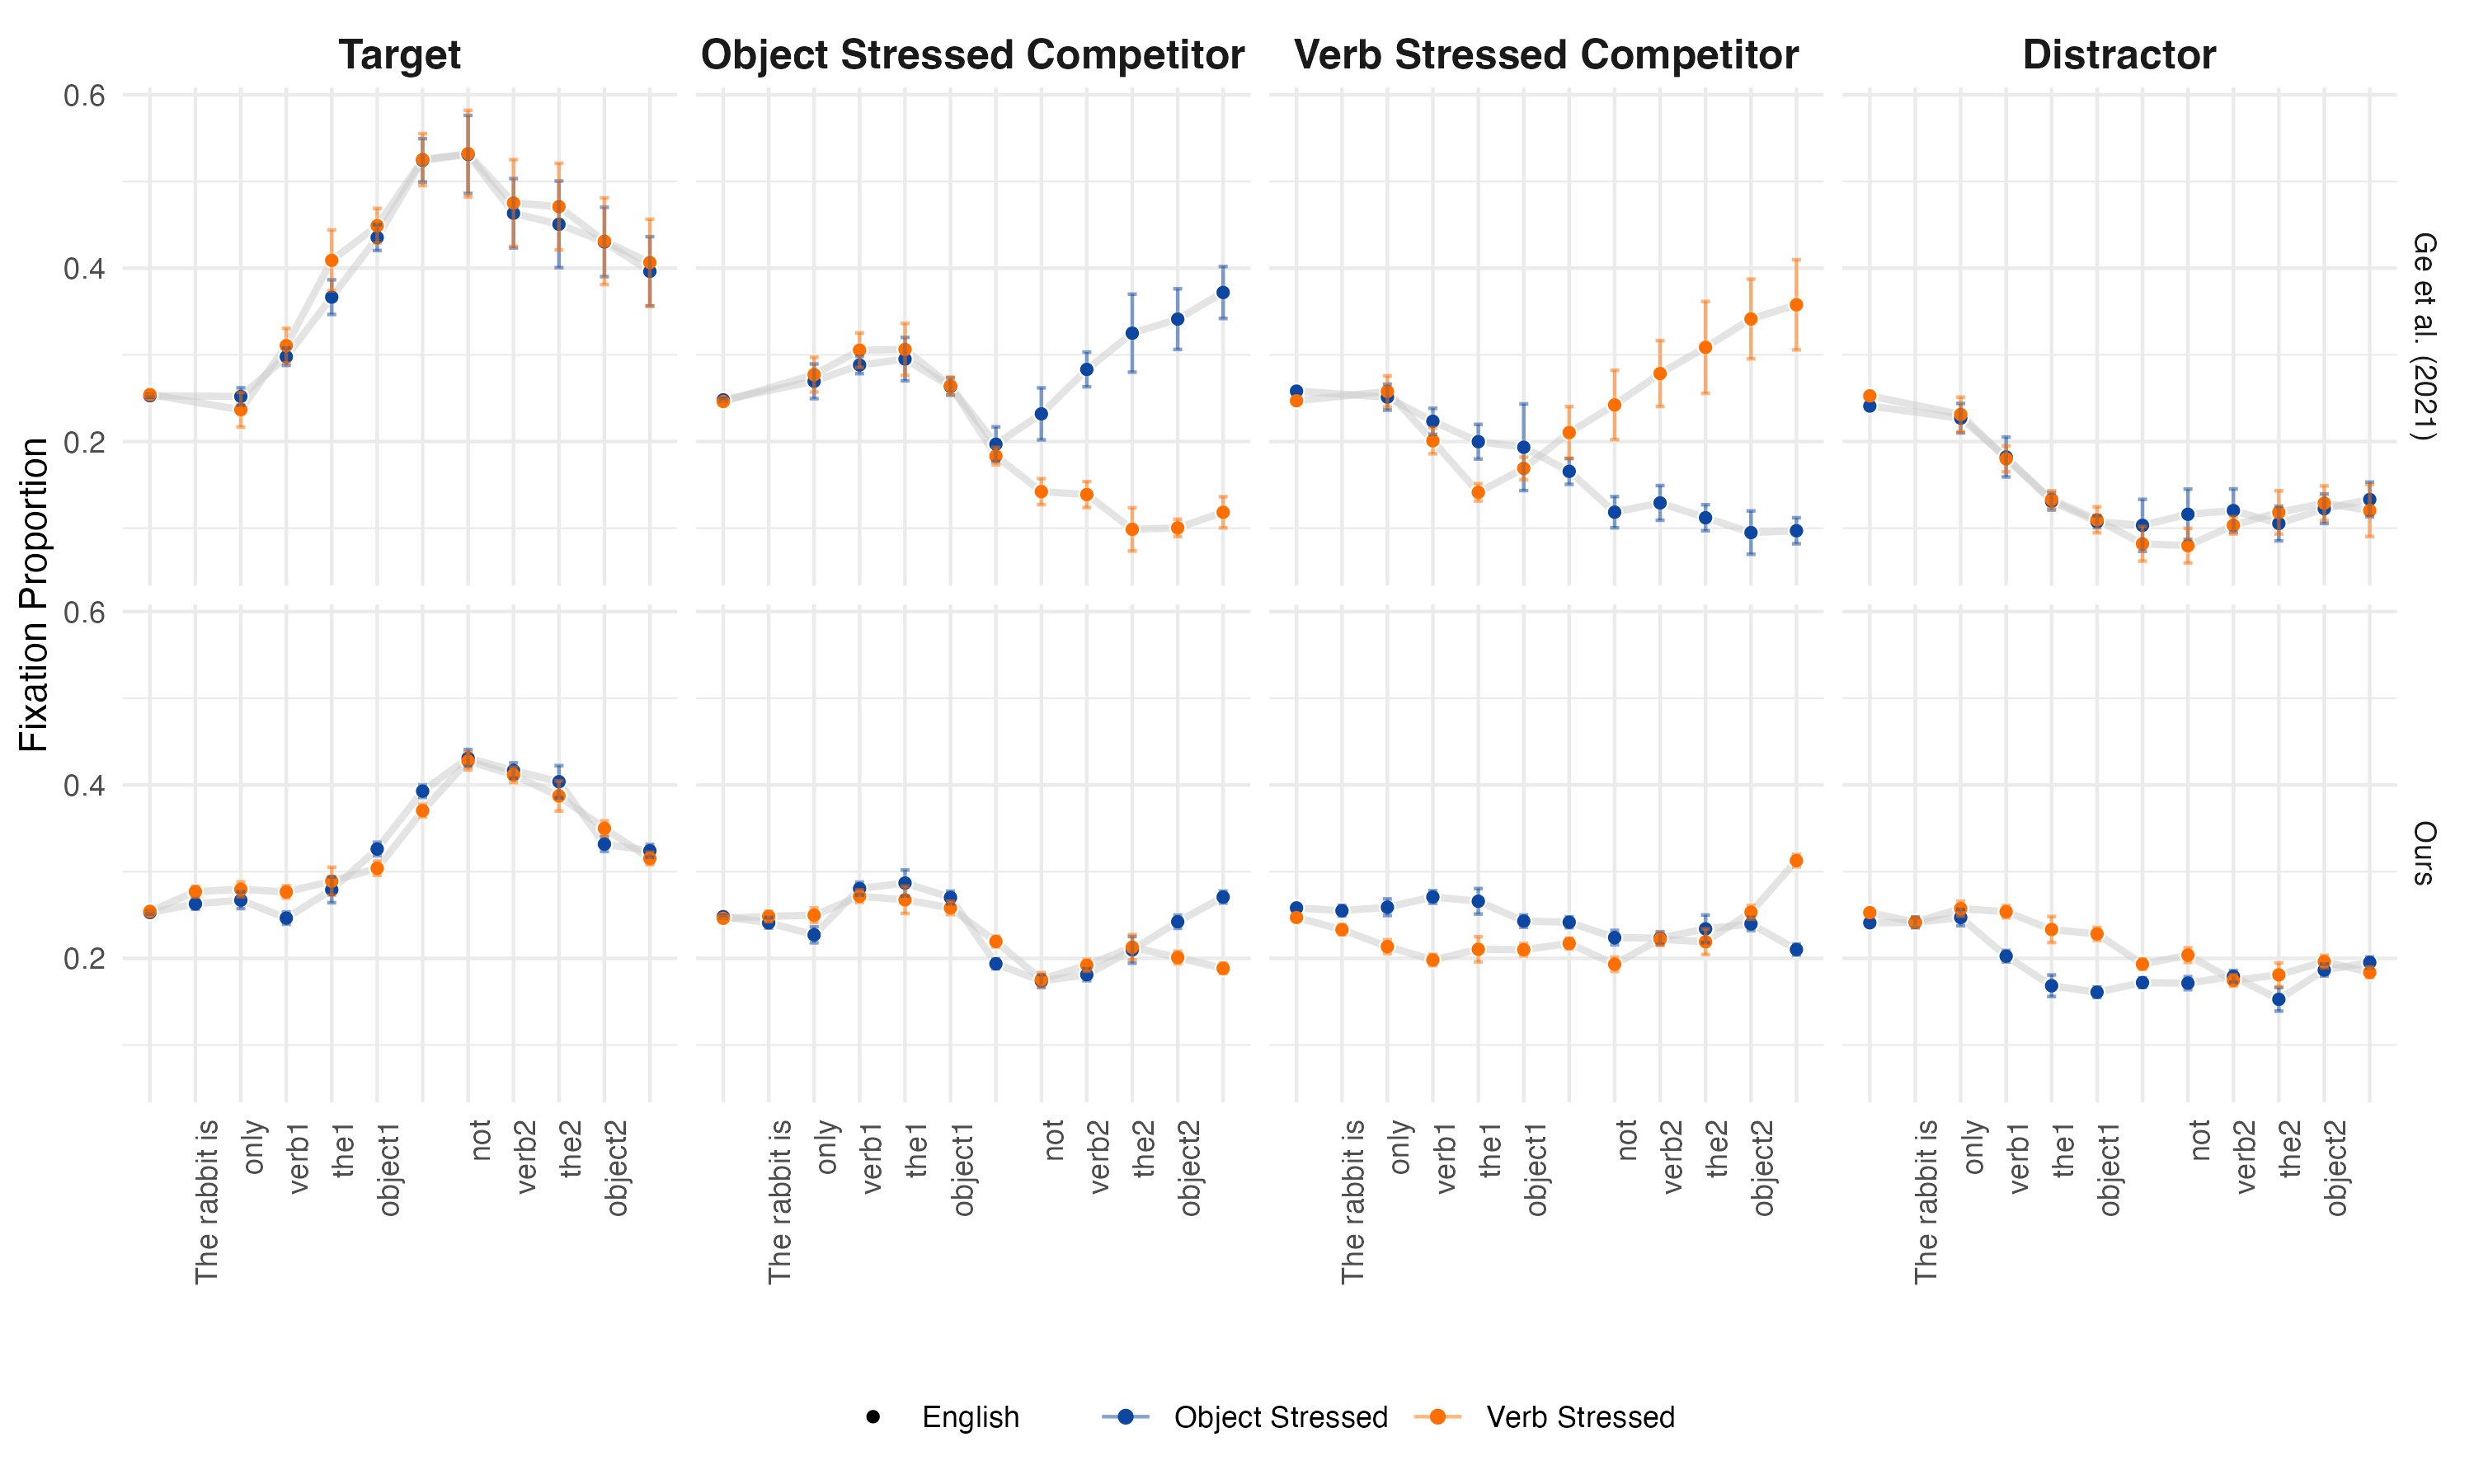
\includegraphics[width=\textwidth,height=\textheight,keepaspectratio]{viz/english_fix.png}
    \caption{things}
    \label{fig:english_fix}
\end{figure}

Unlike Ge et al., our study introduces a web-based data collection method, which necessitated adjustments in participant sampling and eye-tracking calibration. Despite these differences, fixation patterns to the AOIs remained generally consisitent, while the results across the language groups varied substantially, \ref{fig:dutch_fix}

\begin{figure}[H]  % 'p' puts it on its own page
    \centering
    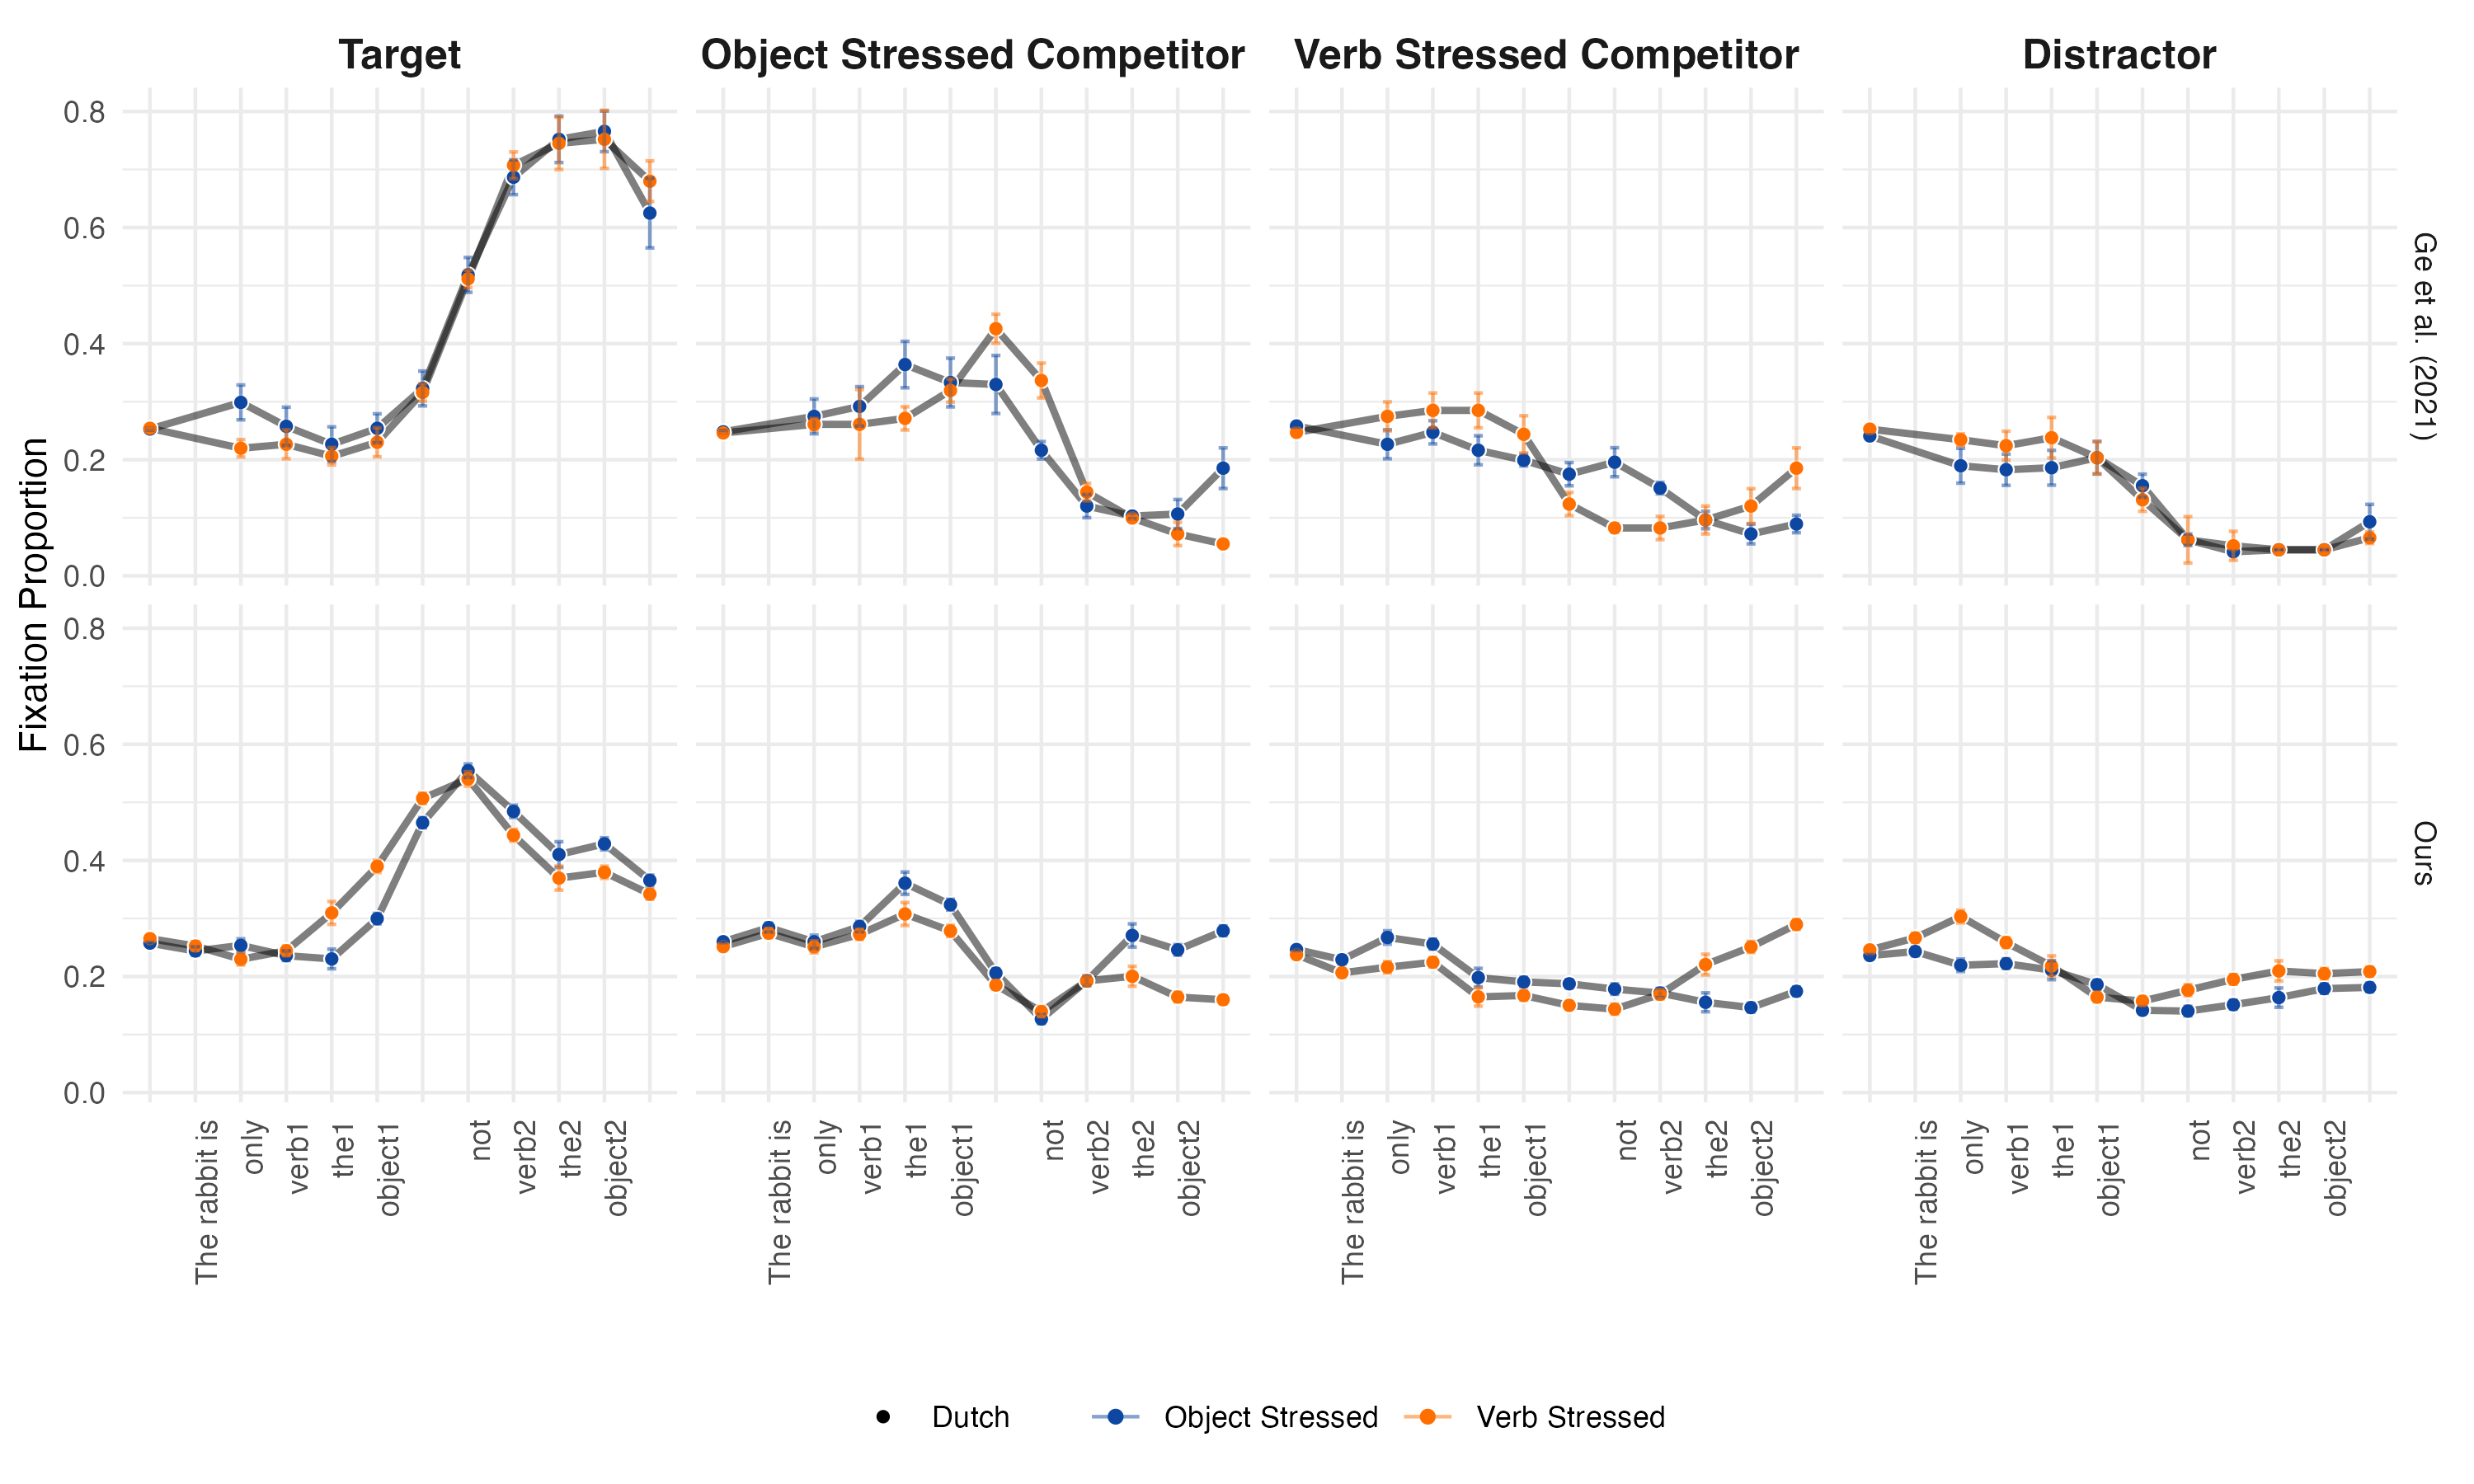
\includegraphics[width=\textwidth,height=\textheight,keepaspectratio]{viz/dutch_fix.png}
    \caption{things}
    \label{fig:dutch_fix}
\end{figure}

Like Ge et al. (2021), we applied mixed-effects regression models to predict fixation proportions as a function of focus condition, time, and area of interest (AOI) for each time bin seperately. We fit a series of linear mixed-effects models (LMMs) with random intercepts for participants and slopes for condition and AOI. The best-fitting models were selected based on lowest AIC. Also like Ge et al. (2021), we used baseline of object stressed for condition and a baseline of object competitor for AOI. This means that negative effects for either can be interpreted as object facing and positive effects are verb facing. Said another way, a positive effect for AOI means more looks toward verb competitor. Likewise, a positive effect for condition indicates more looks during verb focused sentences.

Unlike Ge et al., our model selection pipeline incorporated an automated model comparison approach, iteratively testing models with simpler effects structures. This change was necessary because many models did not converge. The full model includes both AOI and condition, along with their interaction, as well as random intercepts for participant and slopes for item. If this fails to converge or creates a singularity then
this simplifies down to a model that still includes the AOI × condition interaction but removes individual slopes. Next, the interaction between AOI and condition is removed, leaving only the main effects. The model is then further simplified by removing participant-specific effects entirely, keeping just the overall effects of AOI and condition and participant random slopes. If none of these models converge or if the simplest model is the best, then last step is a basic linear model without any participant-level adjustments, treating all data points as independent. This is the simplest possible model. All results will be presented from earlier in the sentence to later.

Results from the 18 statistical tests (9 each for English and Dutch participants) are on competitor fixations. Starting with English models, unlike \citep{Ge2021}, only three main effects were found: A significant positive effect was found for AOI ($\beta$ = 0.062, \textit{SE} = 0.029, \textit{t} = 2.17, \textit{p} = 0.032) indicating more looks to verb competitors than object competitors during the "not" time bin. Further, a signficant positive interaction between AOI and condition was found ($\beta$ = 0.175, \textit{SE} = 0.056, \textit{t} = 3.14, \textit{p} = 0.0019) for the "Offset" time bin, indicating that participants began to look more at the verb competitor during the verb focused sentences. Last, a significant negative effect was found for condition ($\beta$ = -0.091, \textit{SE} = 0.039, \textit{t} = -2.30, \textit{p} = 0.022) indicating more looks to competitors during object focused sentences overall during the offset time bin. Our English participant results can be seen in comparison to Ge et al. (2021) in figure \ref{fig:model_plot_english}

\begin{figure}[H]  % 'p' puts it on its own page
    \centering
    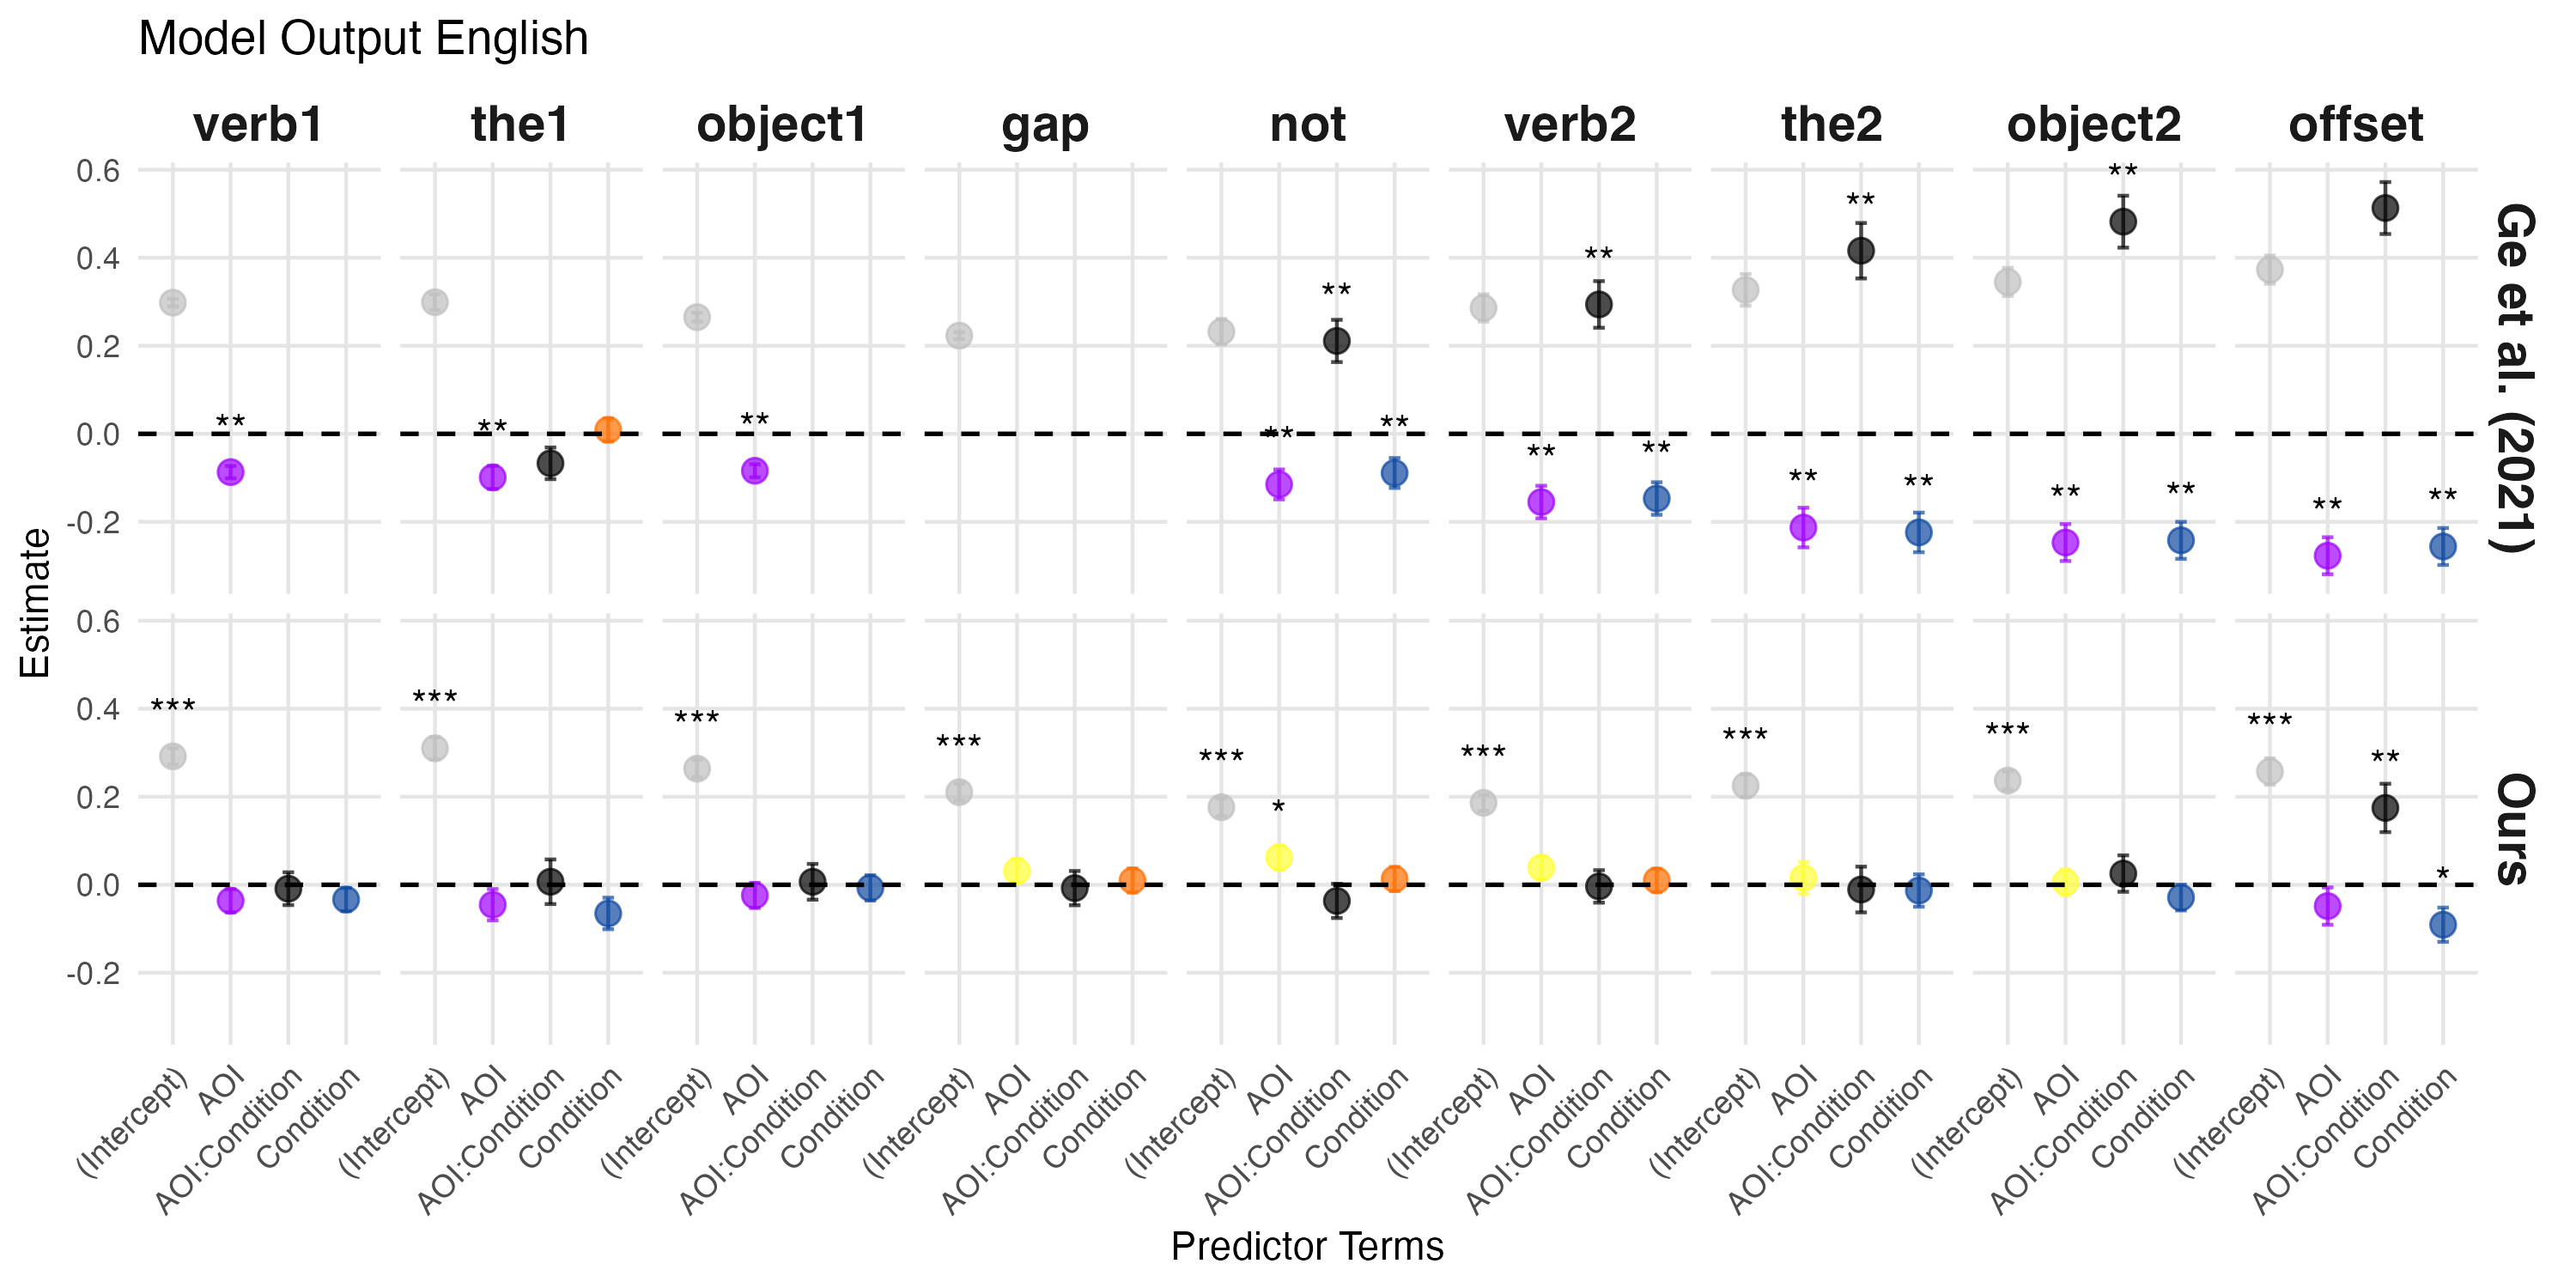
\includegraphics[width=\textwidth,height=\textheight,keepaspectratio]{viz/model_plot_english.png}
    \caption{things}
    \label{fig:model_plot_english}
\end{figure}

For the 9 statistical tests for dutch nine effects were found to be significant. Like before, results will be presented in order of the time bin of the sentence. For "the" time bin, a negative effect of AOI ($\beta$ = -0.099, \textit{SE} = 0.041, \textit{t} = -2.43, \textit{p} = 0.017) was found, indicating more looks to object competitor AOIs. Similarly, negative effect for AOI were found for "object1" ($\beta$ = -0.117, \textit{SE} = 0.033, \textit{t} = -3.59, \textit{p} $<$ 0.001), "the2" ($\beta$ = -0.129, \textit{SE} = 0.042, \textit{t} = -3.08, \textit{p} = 0.0025), and "object2" ($\beta$ = -0.091, \textit{SE} = 0.032, \textit{t} = -2.83, \textit{p} = 0.0055) timebins , all indicating more looks to the object competitors AOIs. Further, a negative effect of condition was found for both "object2" ($\beta$ = 0.180, \textit{SE} = 0.045, \textit{t} = 3.98, \textit{p} $<$ 0.001) and "offset" ($\beta$ = -0.130, \textit{SE} = 0.050, \textit{t} = -2.58, \textit{p} = 0.011), indicating more looks to competitors during verb focused sentences. Lastly, a positive interaction between AOI and condition was found during the "object2" ($\beta$ = 0.180, \textit{SE} = 0.045, \textit{t} = 3.98, \textit{p} $<$ 0.001) and "offset" ($\beta$ = 0.226, \textit{SE} = 0.071, \textit{t} = 3.17, \textit{p} = 0.0019)
time bins, indicating more looks to object competitors during object focused sentences. Our Dutch participant results can be seen in comparison to Ge et al. (2021) in figure \ref{fig:model_plot_english}


\begin{figure}[H]  % 'p' puts it on its own page
    \centering
    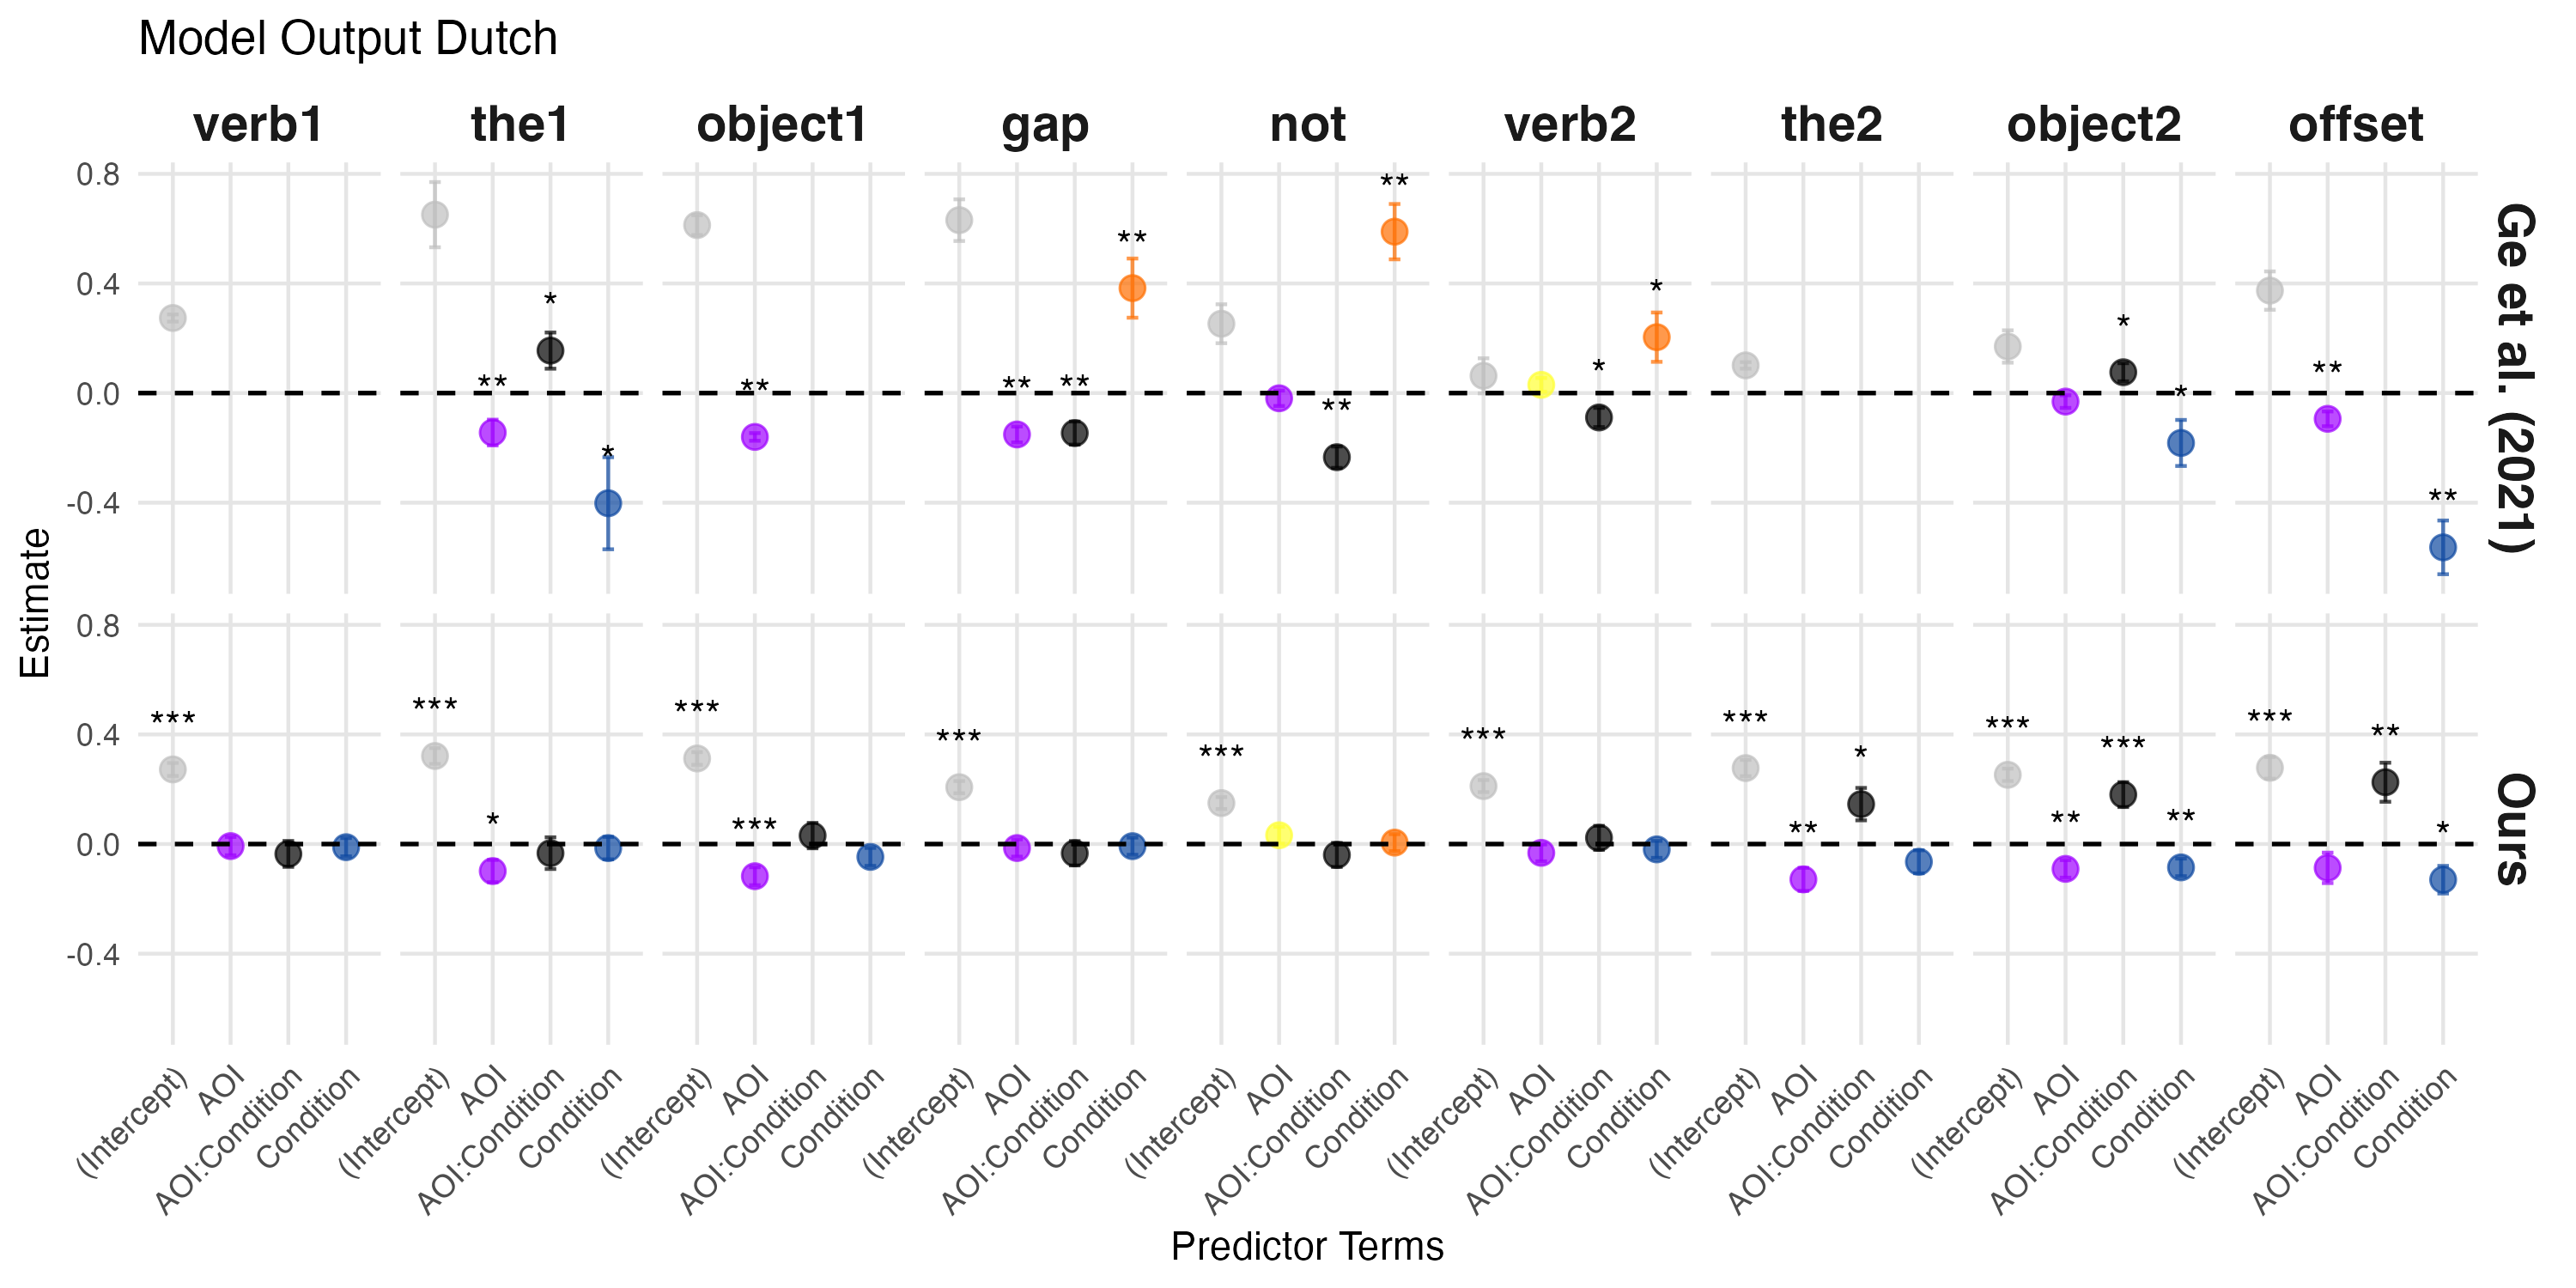
\includegraphics[width=\textwidth,height=\textheight,keepaspectratio]{viz/model_plot_dutch.png}
    \caption{modle ouutputs for Dutch participants across modeled time bin. Order of time bins appears in order across the top.   Estimates of \citep{Ge2021} data appears on top while Our data}
    \label{fig:model_plot_dutch}
\end{figure}


\subsubsection{Methodological refinement: A "focused" approach}

While fidelity in replication is essential, it is also necessary to evaluate whether the original analytical choices align with current best practices. The refinement phase of our analysis serves to enhance statistical rigor by addressing potential limitations such as model specification, overfitting, multiple comparisons, and analytical transparency.

Here, we implement refined statistical approaches that maintain the interpretability of the original findings while increasing robustness. This includes evaluating model assumptions, testing alternative specifications that account for variance more effectively, and applying more conservative corrections to reduce the likelihood of Type I errors. By implementing these refinements, we ensure that our results reflect genuine patterns in the data rather than artifacts of less stringent analytical choices.

These refinements do not alter the core structure of the replication but rather provide a more precise and statistically rigorous evaluation of the original claims. By comparing our refined results to both the original and replicated findings, we can assess whether methodological improvements impact the observed effects and whether the key conclusions of \citep{Ge2021} remain stable across different analytical approaches.

The first refinement that we do is that we compare not only competitor fixation but we also compare target fixations. We do this in hopes to have a more wholistic perspective on the participants behavior. Secondly, we combine the analysis form both language groups to be able to compare both within language by conditino and across participant L1. Fig \ref{fig:english_fix2} shows a more interpretable version of \ref{fig:english_fix}, which allows you to compare when fixations to specific AOI begin to deviate from each other not just across condition.

\begin{figure}[H]  % 'p' puts it on its own page
    \centering
    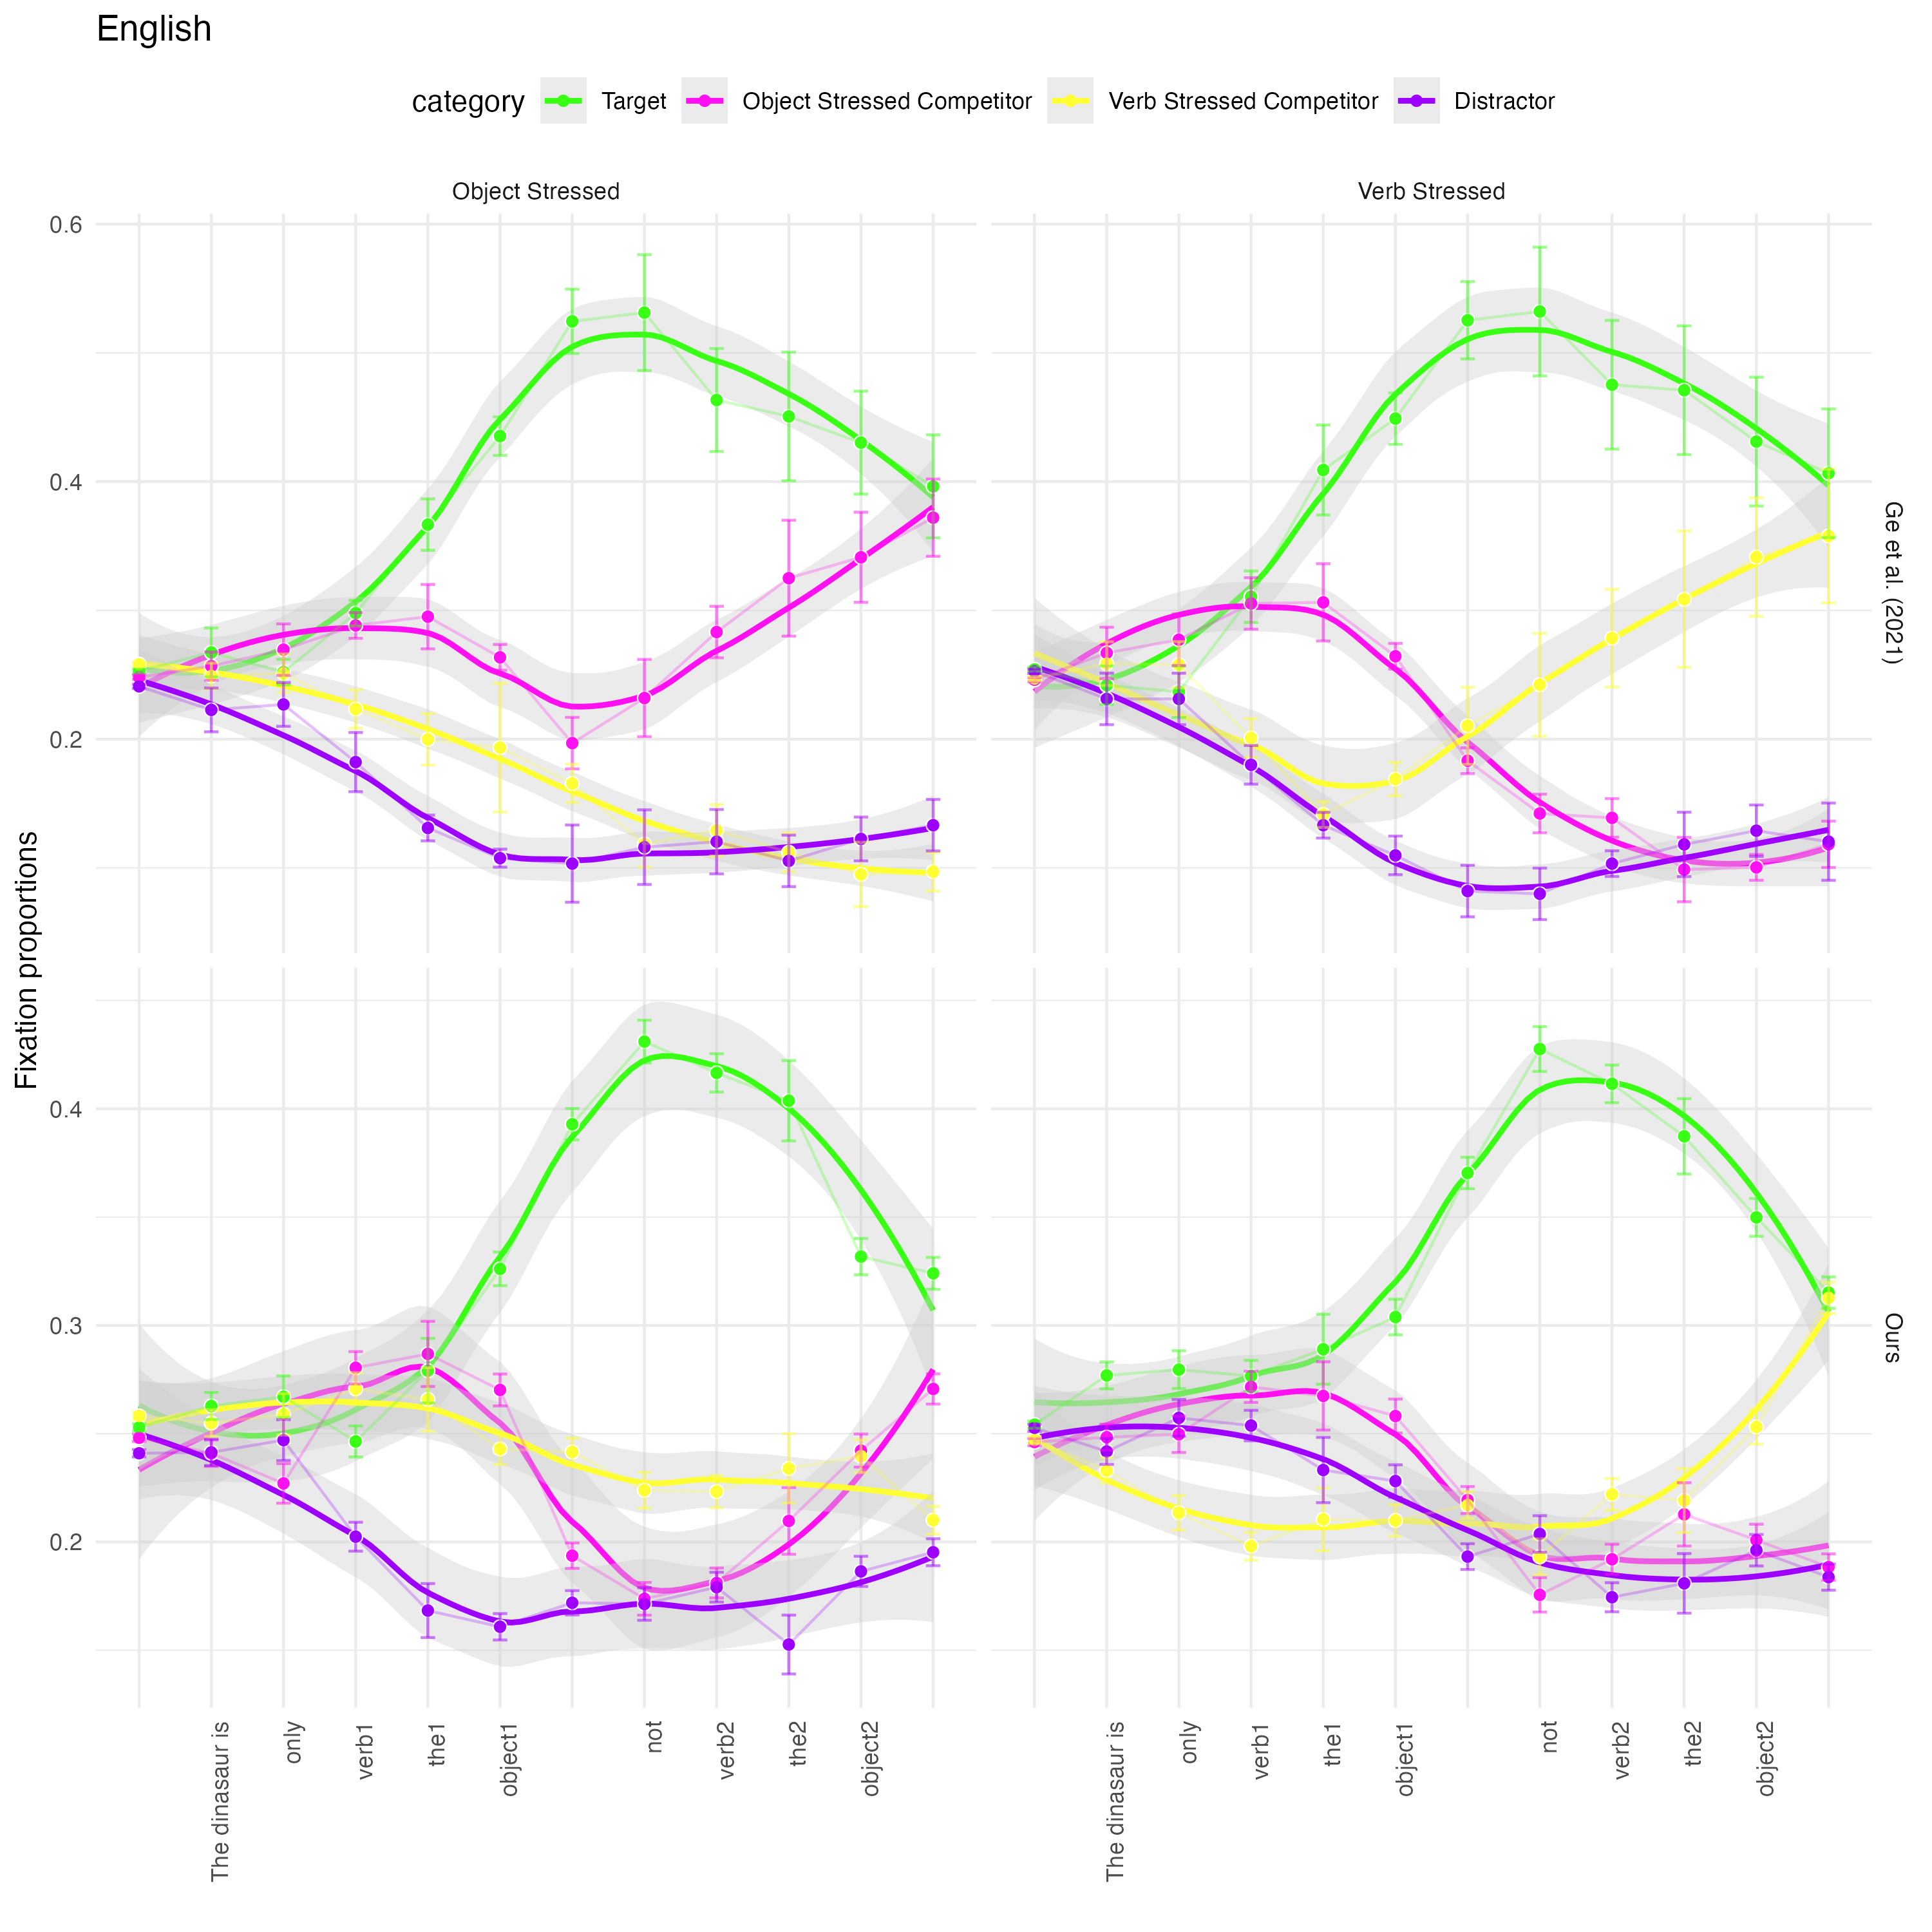
\includegraphics[width=\textwidth,height=\textheight,keepaspectratio]{viz/english_fix2.png}
    \caption{fixation proportions for English participants across object stressed (left) and verb stressed (right) sentences. Estimates of \citep{Ge2021} data appears on top while Our data appears below}
    \label{fig:english_fix2}
\end{figure}

For these refined models, we have both a target models and a competitor models. That is, we are comparing the target fixations (green lines in figures figures \ref{fig:english_fix2} and \ref{fig:dutch_fix2}) in the target model and we are comparing the object competitor fixations (yellow lines in figures \ref{fig:english_fix2} and \ref{fig:dutch_fix2}) in the object focused sentences (left plots of figures \ref{fig:english_fix2} and \ref{fig:dutch_fix2}) as well as the verb competitor fixations (purple lines in figures \ref{fig:english_fix2} and \ref{fig:dutch_fix2}) during verb focused sentences (right plots of figures \ref{fig:english_fix2} and \ref{fig:dutch_fix2})) for the competitor models. 

\begin{figure}[H]  % 'p' puts it on its own page
    \centering
    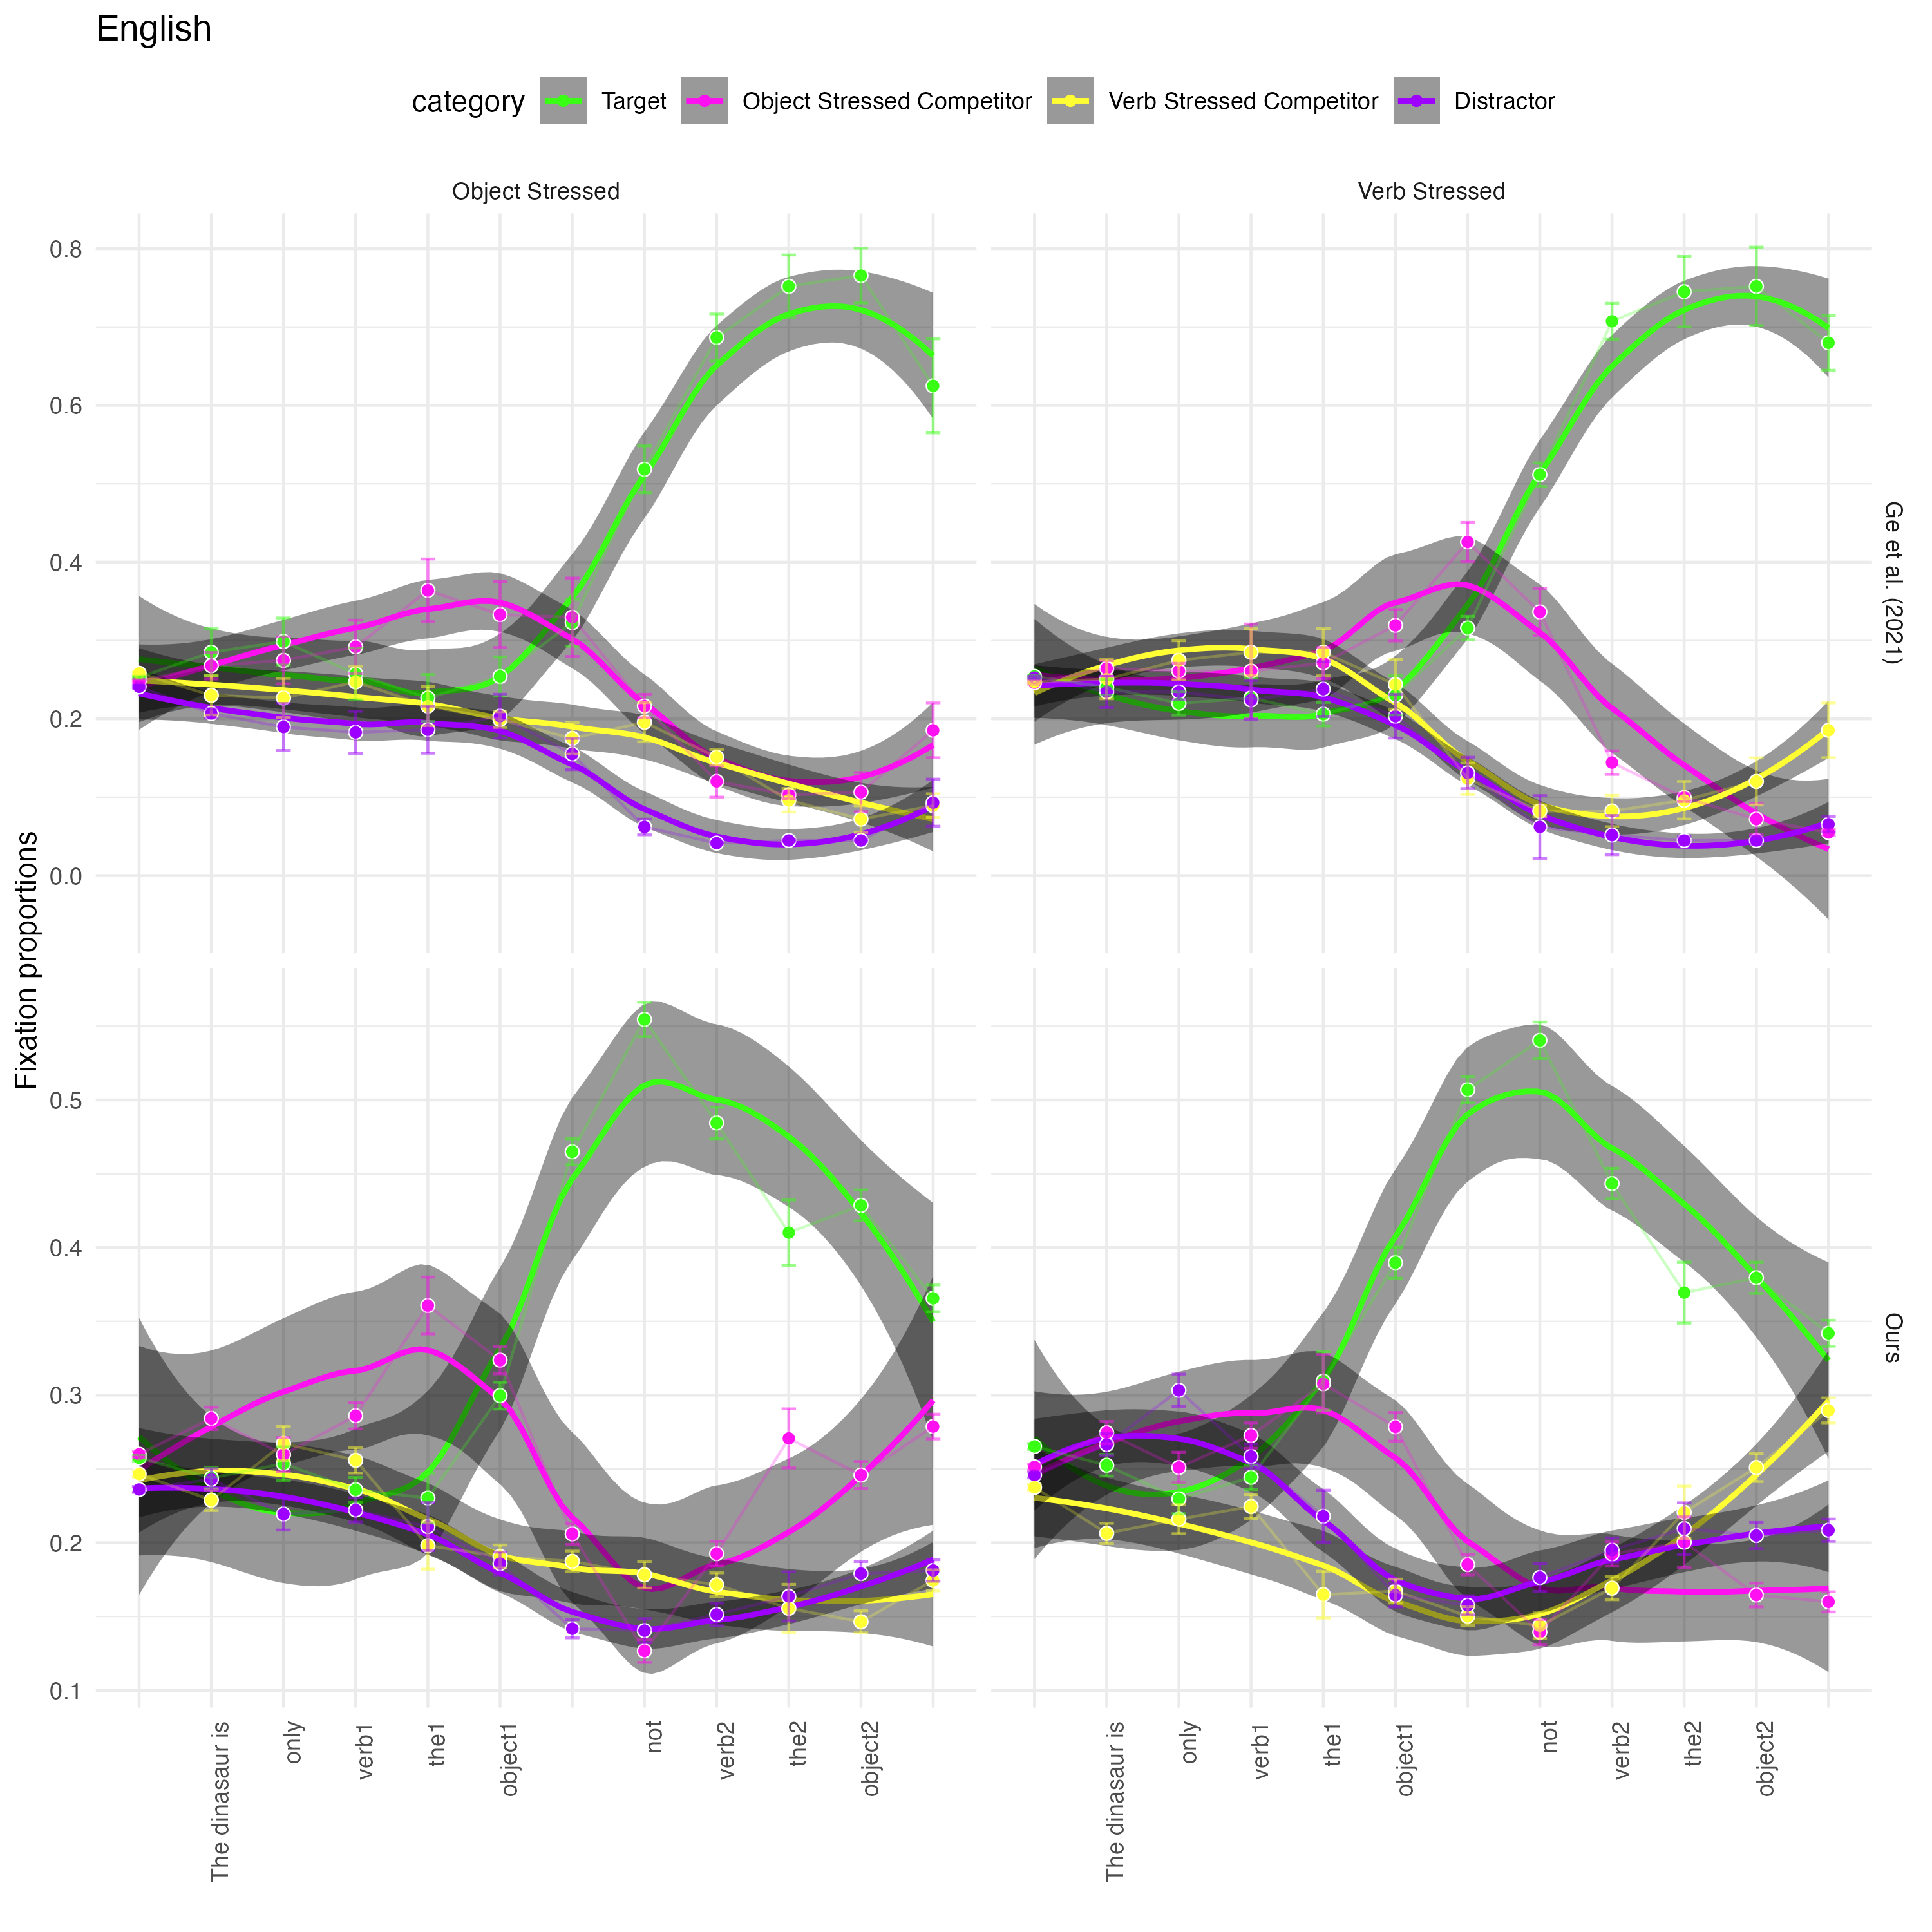
\includegraphics[width=\textwidth,height=\textheight,keepaspectratio]{viz/dutch_fix2.png}
    \caption{fixation proportions for Dutch participants across object stressed (left) and verb stressed (right) sentences. Estimates of \citep{Ge2021} data appears on top while Our data appears below}
    \label{fig:dutch_fix2}
\end{figure}

An additional difference in our refined model is that we do all time bins in a single model. However, we split the sentence at the gap between the first phrase(e.g., "the rabbit only verb1 the1 object1) and second phrase (e.g., "not verb2 the2 object2). 

Unlike the linear mixed-effects models (LMMs) used in the fidelity modeling, this stage applies Generalized Additive Models (GAMs) to better capture time-dependent changes in fixation proportions. Since eye-tracking data unfolds continuously over time, GAMs provide a more flexible way to model the nonlinear dynamics of fixations that may not be well captured by traditional LMMs. In this approach, we compare two GAM variants: a full interaction model, which includes a three-way interaction between time, experiment group, and condition, and a main effects model, which assumes that changes in fixation proportions follow an additive pattern without time-dependent interactions. Both models include random smooth effects for participants, allowing for individual variability while capturing group-level fixation trends. Max models started with random items as well but none converged.

To determine the best-fitting model, we use BIC, where lower values indicate a better model fit. Unlike LMMs, which assume linear relationships between predictors and fixation proportions, GAMs allow for smooth, nonlinear changes over time, making them particularly well-suited for tracking how fixations dynamically evolve in response to prosodic cues. By using GAMs, we ensure that our analysis captures fine-grained temporal patterns in visual attention that might be overlooked by standard mixed-effects models.

Results of our 4 models (target-competitor models and phrase 1-phrase 2) are as follows. For the first phrase of the target models a positive main effect stress was found ($\beta$ = 0.155, \textit{SE} = 0.053, \textit{t} = 2.93, \textit{p} = 0.0034) indicating more target fixations during object focus sentences. This effect is somewhat attenuated by the negative interaction between time and stress in phrase 1 of the target model ($\beta$ = -0.036, \textit{SE} = 0.017, \textit{t} = -2.12, \textit{p} = 0.034), indicating more verb looks to targets later on in phrase one for verb focused sentences. During the second phrase, a negative interaction between L1 and time ($\beta$ = -0.058, \textit{SE} = 0.019, \textit{t} = -3.09, \textit{p} = 0.002) indicates more looks to targets for English L1 participants.

For the competitor model first phrase model, a negative interaction between time and stress was found ($\beta$ = -0.095, \textit{SE} = 0.018, \textit{t} = -5.26, \textit{p} $$<$$ 0.001), indicating more looks to verb competitors as time increases. No significant effects were found for the second phrase competitor model.


\begin{figure}[H]  % 'p' puts it on its own page
    \centering
    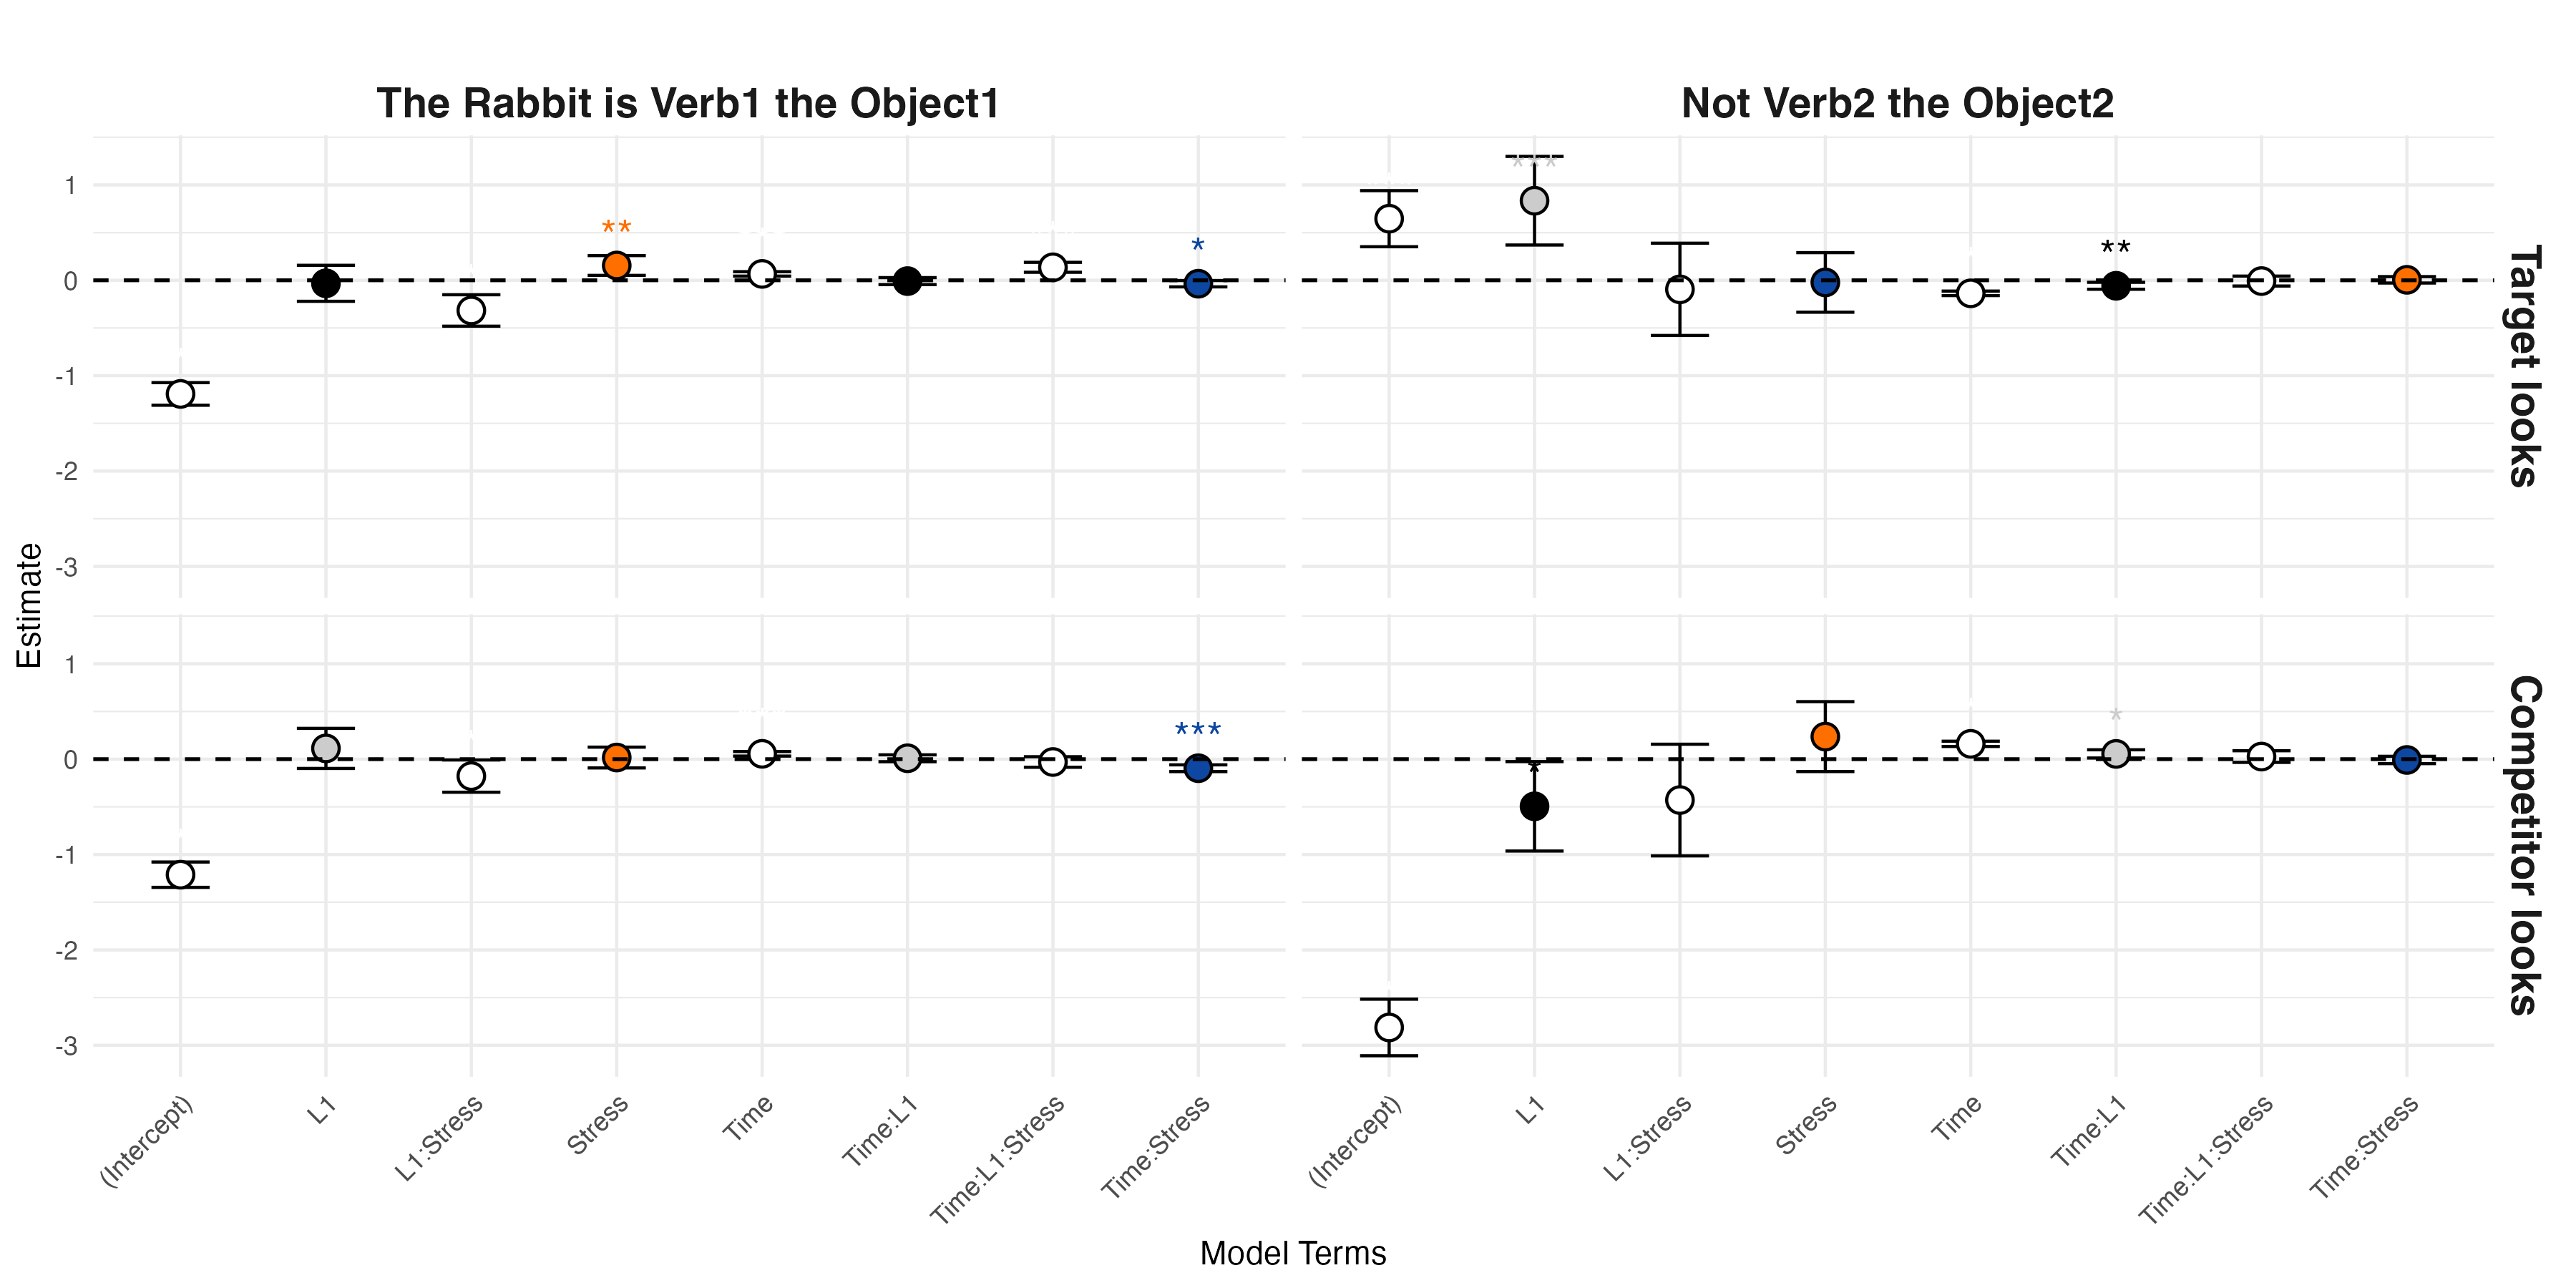
\includegraphics[width=\textwidth,height=\textheight,keepaspectratio]{viz/gam_mod_out.png}
    \caption{things}
    \label{fig:gam_mod_out}
\end{figure}

\subsection{Extension}

Beyond replication and refinement, we extend the analysis to explore additional theoretical questions not examined in \citep{Ge2021}. While the original study provided insights into focus processing, it did not explicitly investigate whether individual cognitive and perceptual differences influence listener behavior. Given prior research suggesting that factors such as working memory, auditory perception, and cognitive control contribute to language processing variability, we test whether these factors modulate eye-movement patterns in response to focus cues. Individual difference between our partiicpants can be found in figure \ref{fig:combined_plot}. In this plot we attempt to show a full picture of the multifaceted dimensions of 

\clearpage
\begin{figure}[p]  % 'p' puts it on its own page
    \centering
    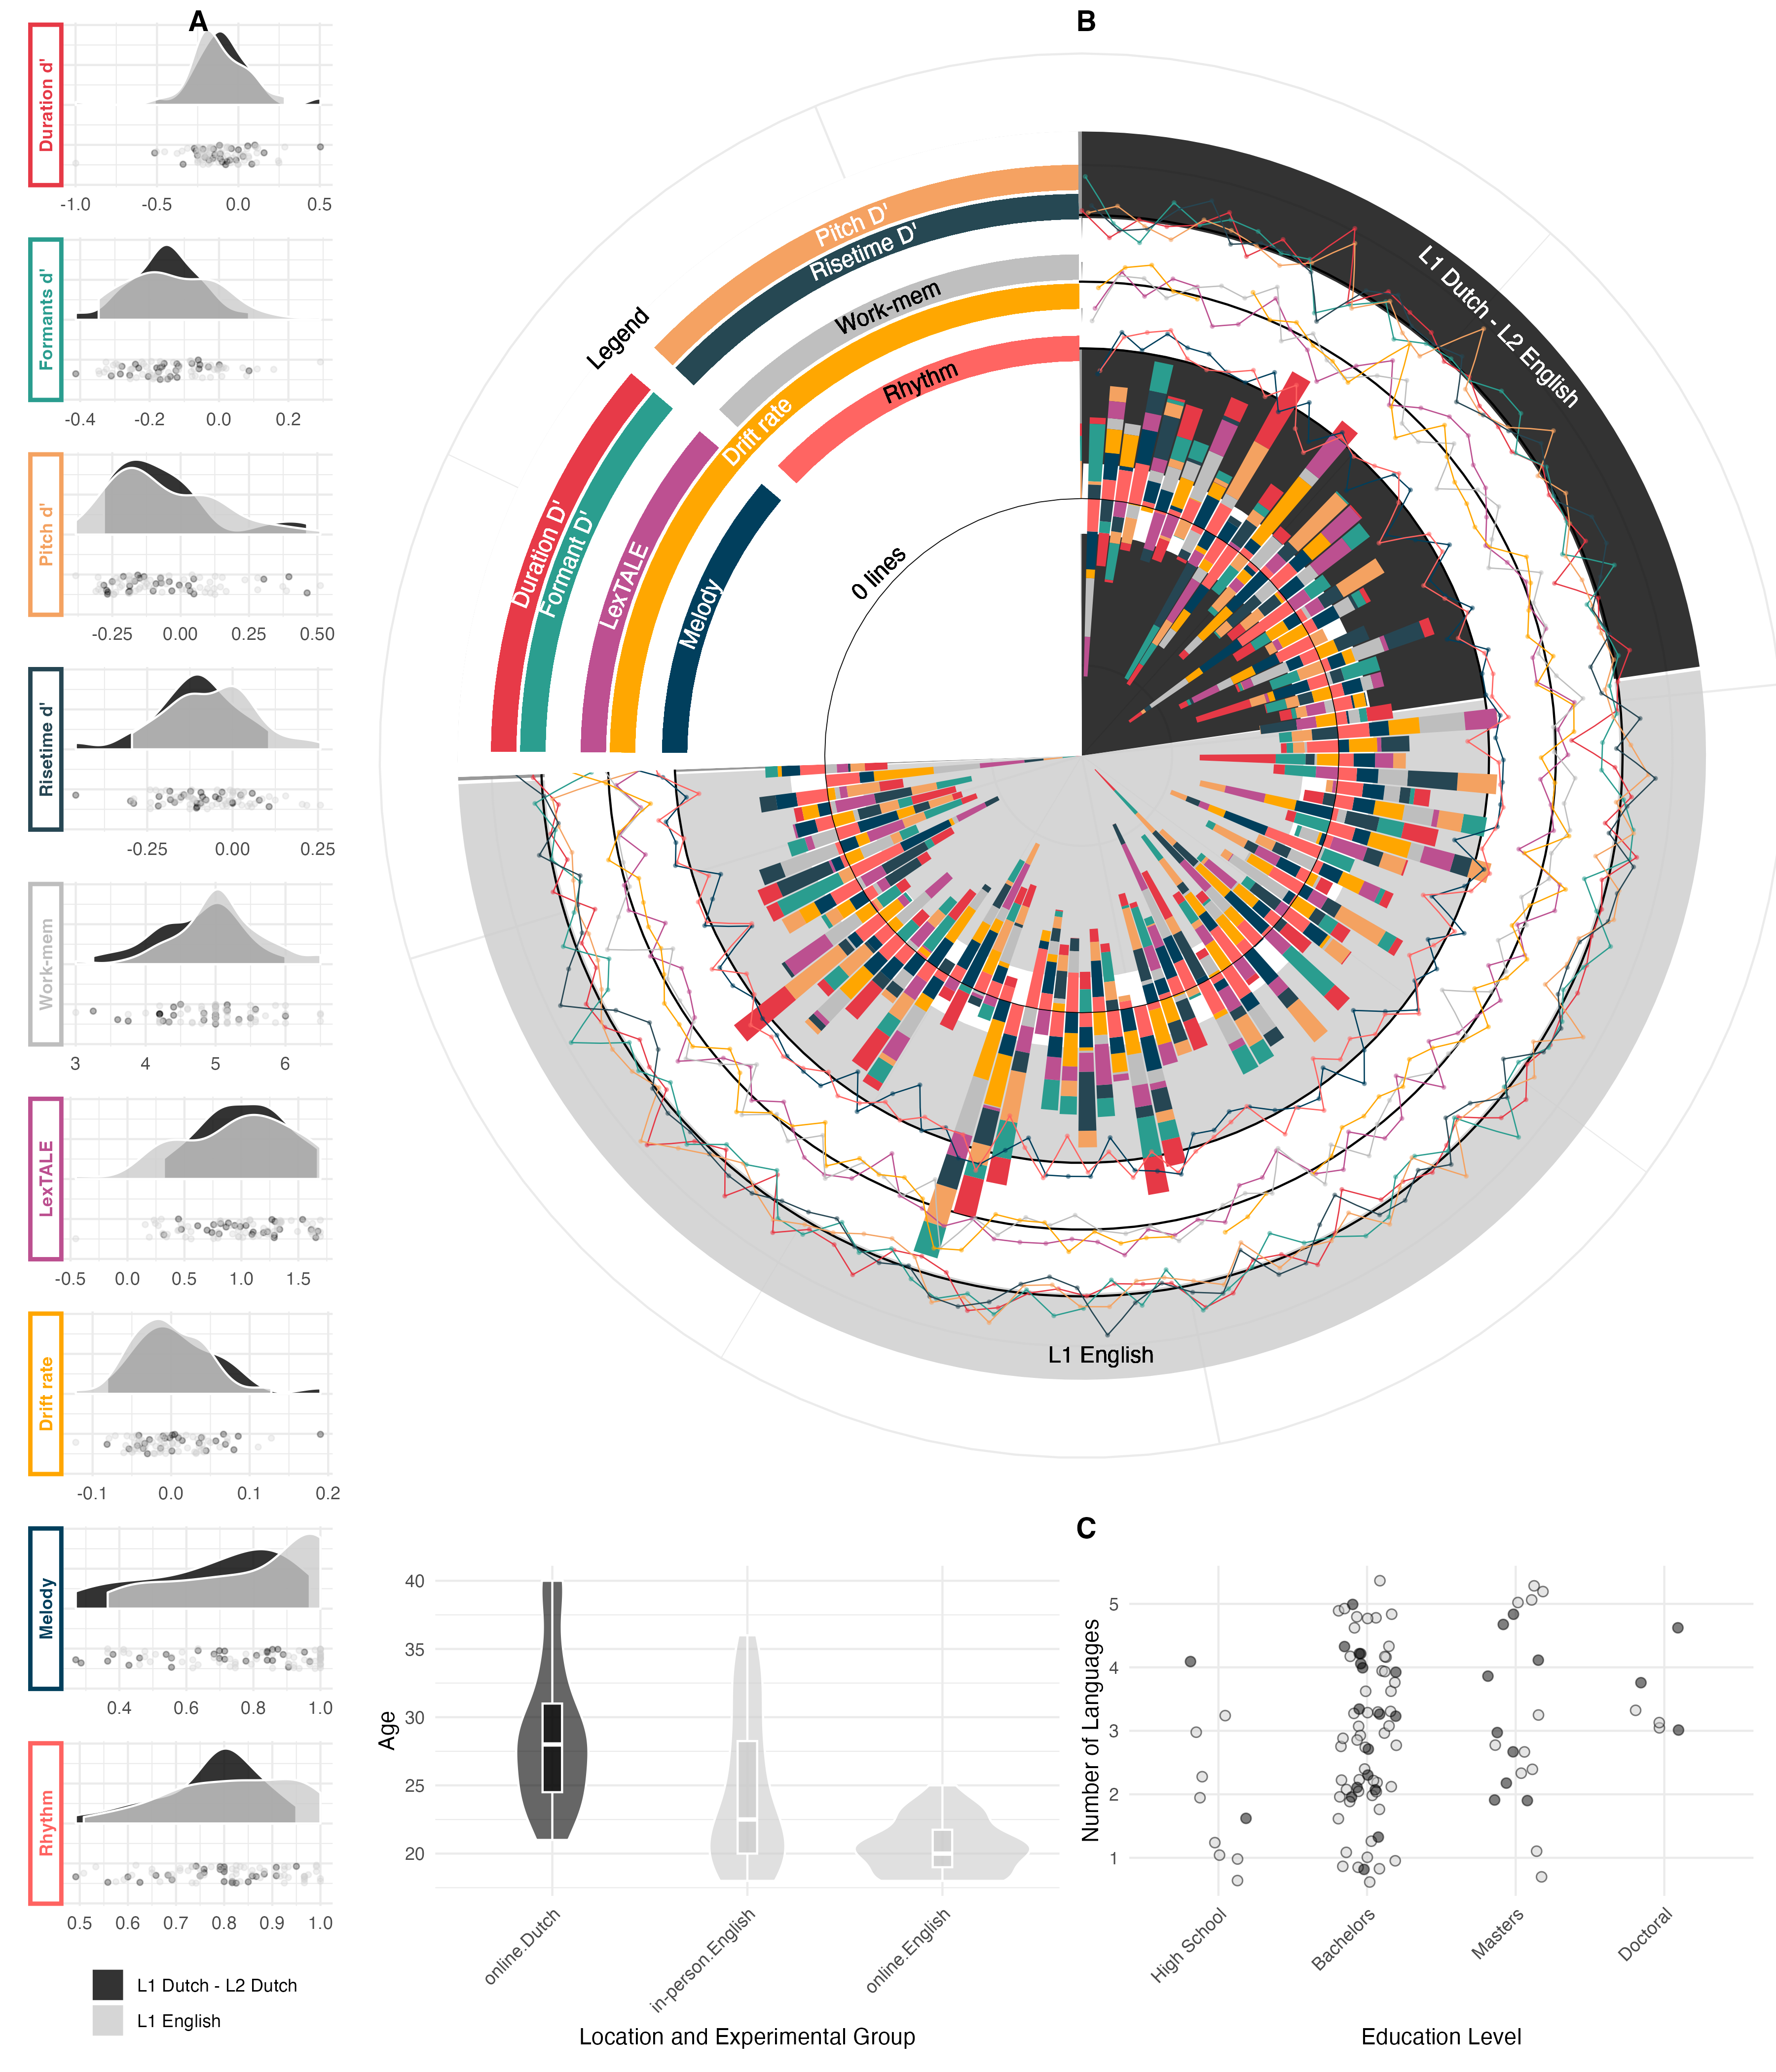
\includegraphics[width=\textwidth,height=\textheight,keepaspectratio]{viz/combined_plot_circle.png}
    \caption{describe what is going on here- A- tasks across the Dutch and English, B individual difference vectors for each participant, C background information on participants}
    \label{fig:combined_plot}
\end{figure}
\clearpage


Addi

This exploratory extension allows us to assess the generalizability of the original findings by considering sources of variability that were not accounted for in the original study. Unlike the fidelity and refinement analyses, which adhere to confirmatory statistical approaches, this extension adopts a theory-driven, exploratory framework. We incorporate measures of lexical proficiency, auditory sensitivity, and motor reproduction ability to determine whether individual cognitive and perceptual traits predict variation in focus processing.

By adopting this three-tiered approach—fidelity, refinement, and extension—we provide a comprehensive analysis that both evaluates and expands upon the findings of \citep{Ge2021}. In what follows, we first present the results of our close replication, followed by methodological refinements, and finally, our exploratory analyses of individual differences.

acoustics:
\begin{figure}[H]  % 'p' puts it on its own page
    \centering
    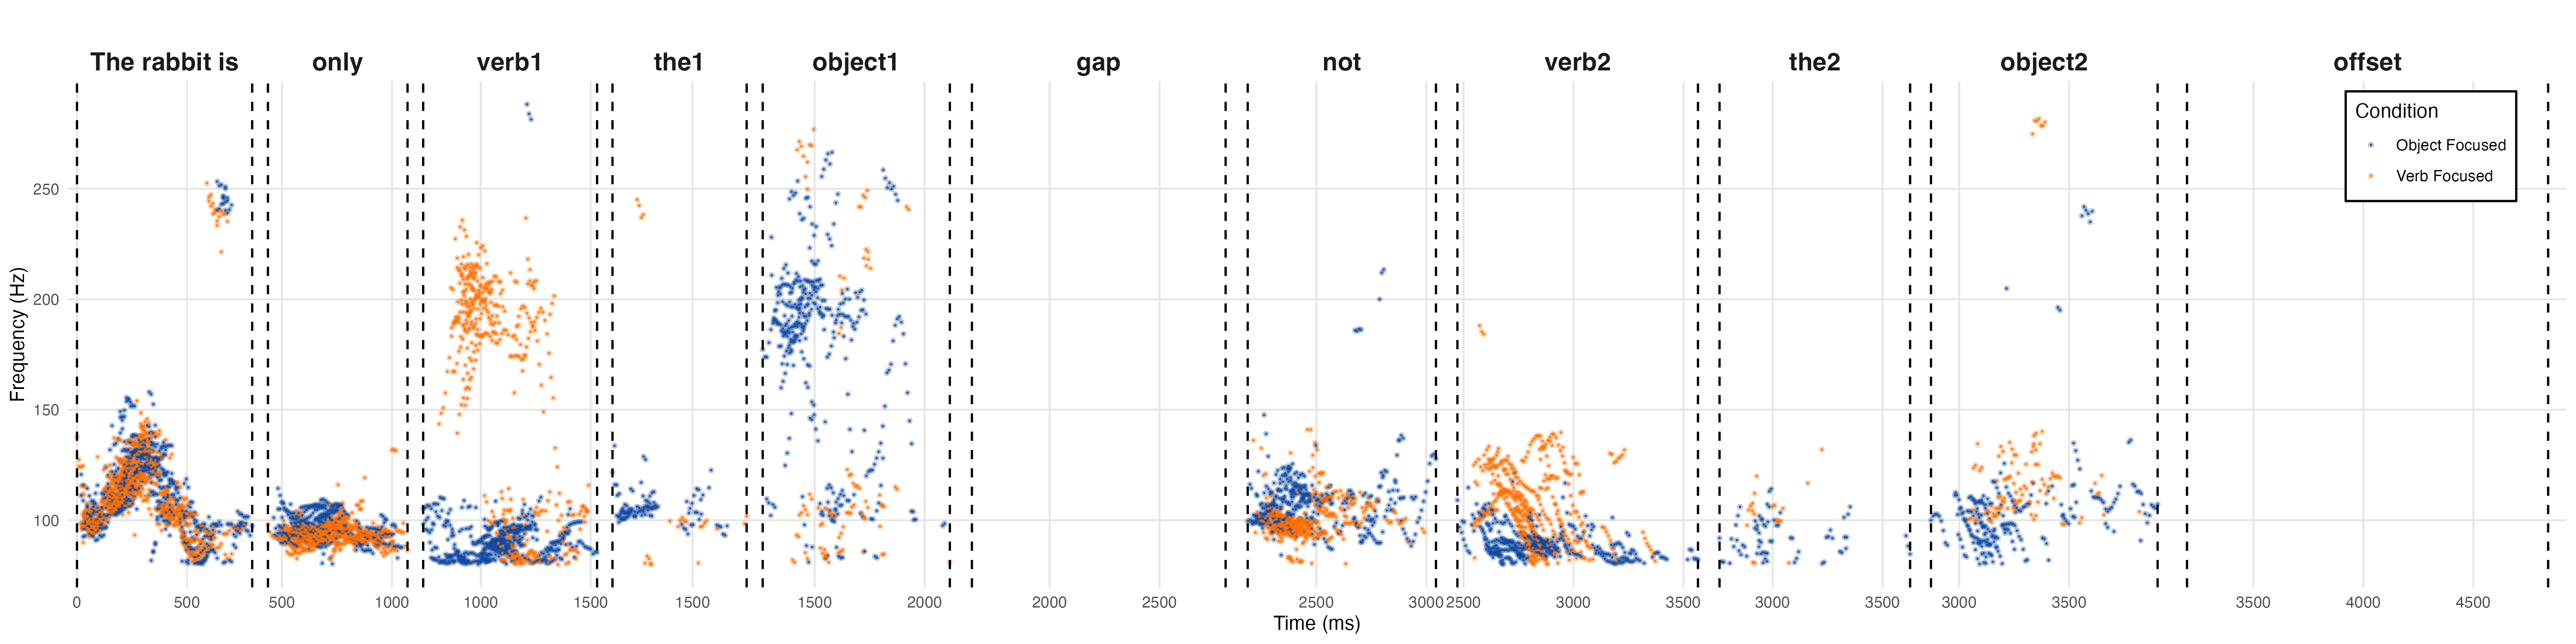
\includegraphics[width=\textwidth,height=\textheight,keepaspectratio]{viz/accoustic.png}
    \caption{things}
    \label{fig:acoustic}
\end{figure}

\begin{figure}[H]  % 'p' puts it on its own page
    \centering
    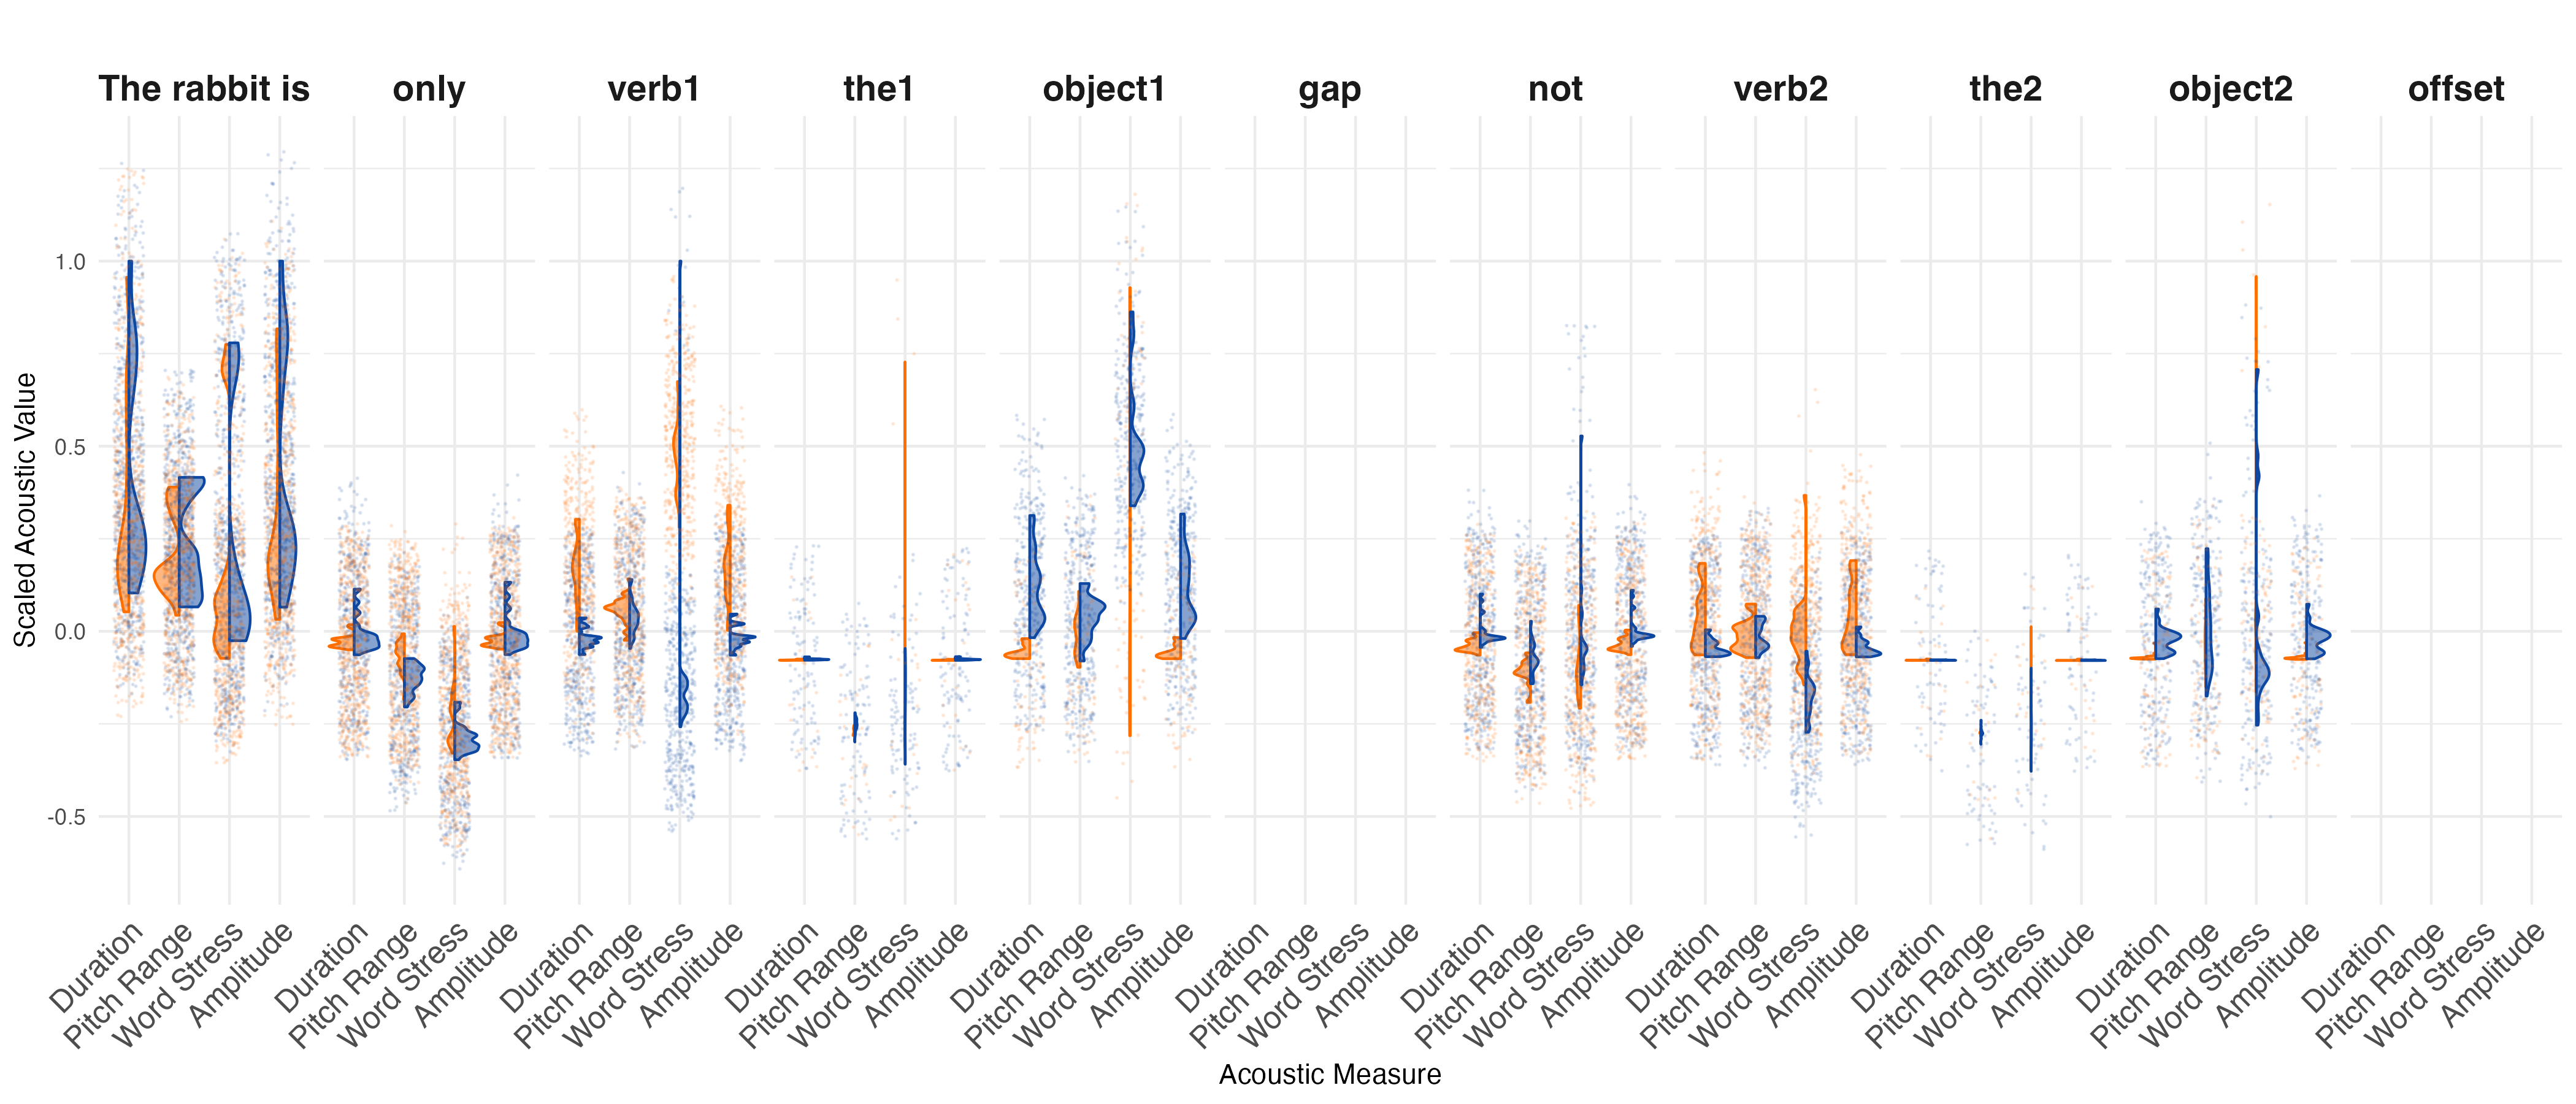
\includegraphics[width=\textwidth,height=\textheight,keepaspectratio]{viz/acoustic_faceted.png}
    \caption{things}
    \label{fig:acoustic_faceted}
\end{figure}



Individual difference plot:


\begin{figure}[H]  % 'p' puts it on its own page
    \centering
    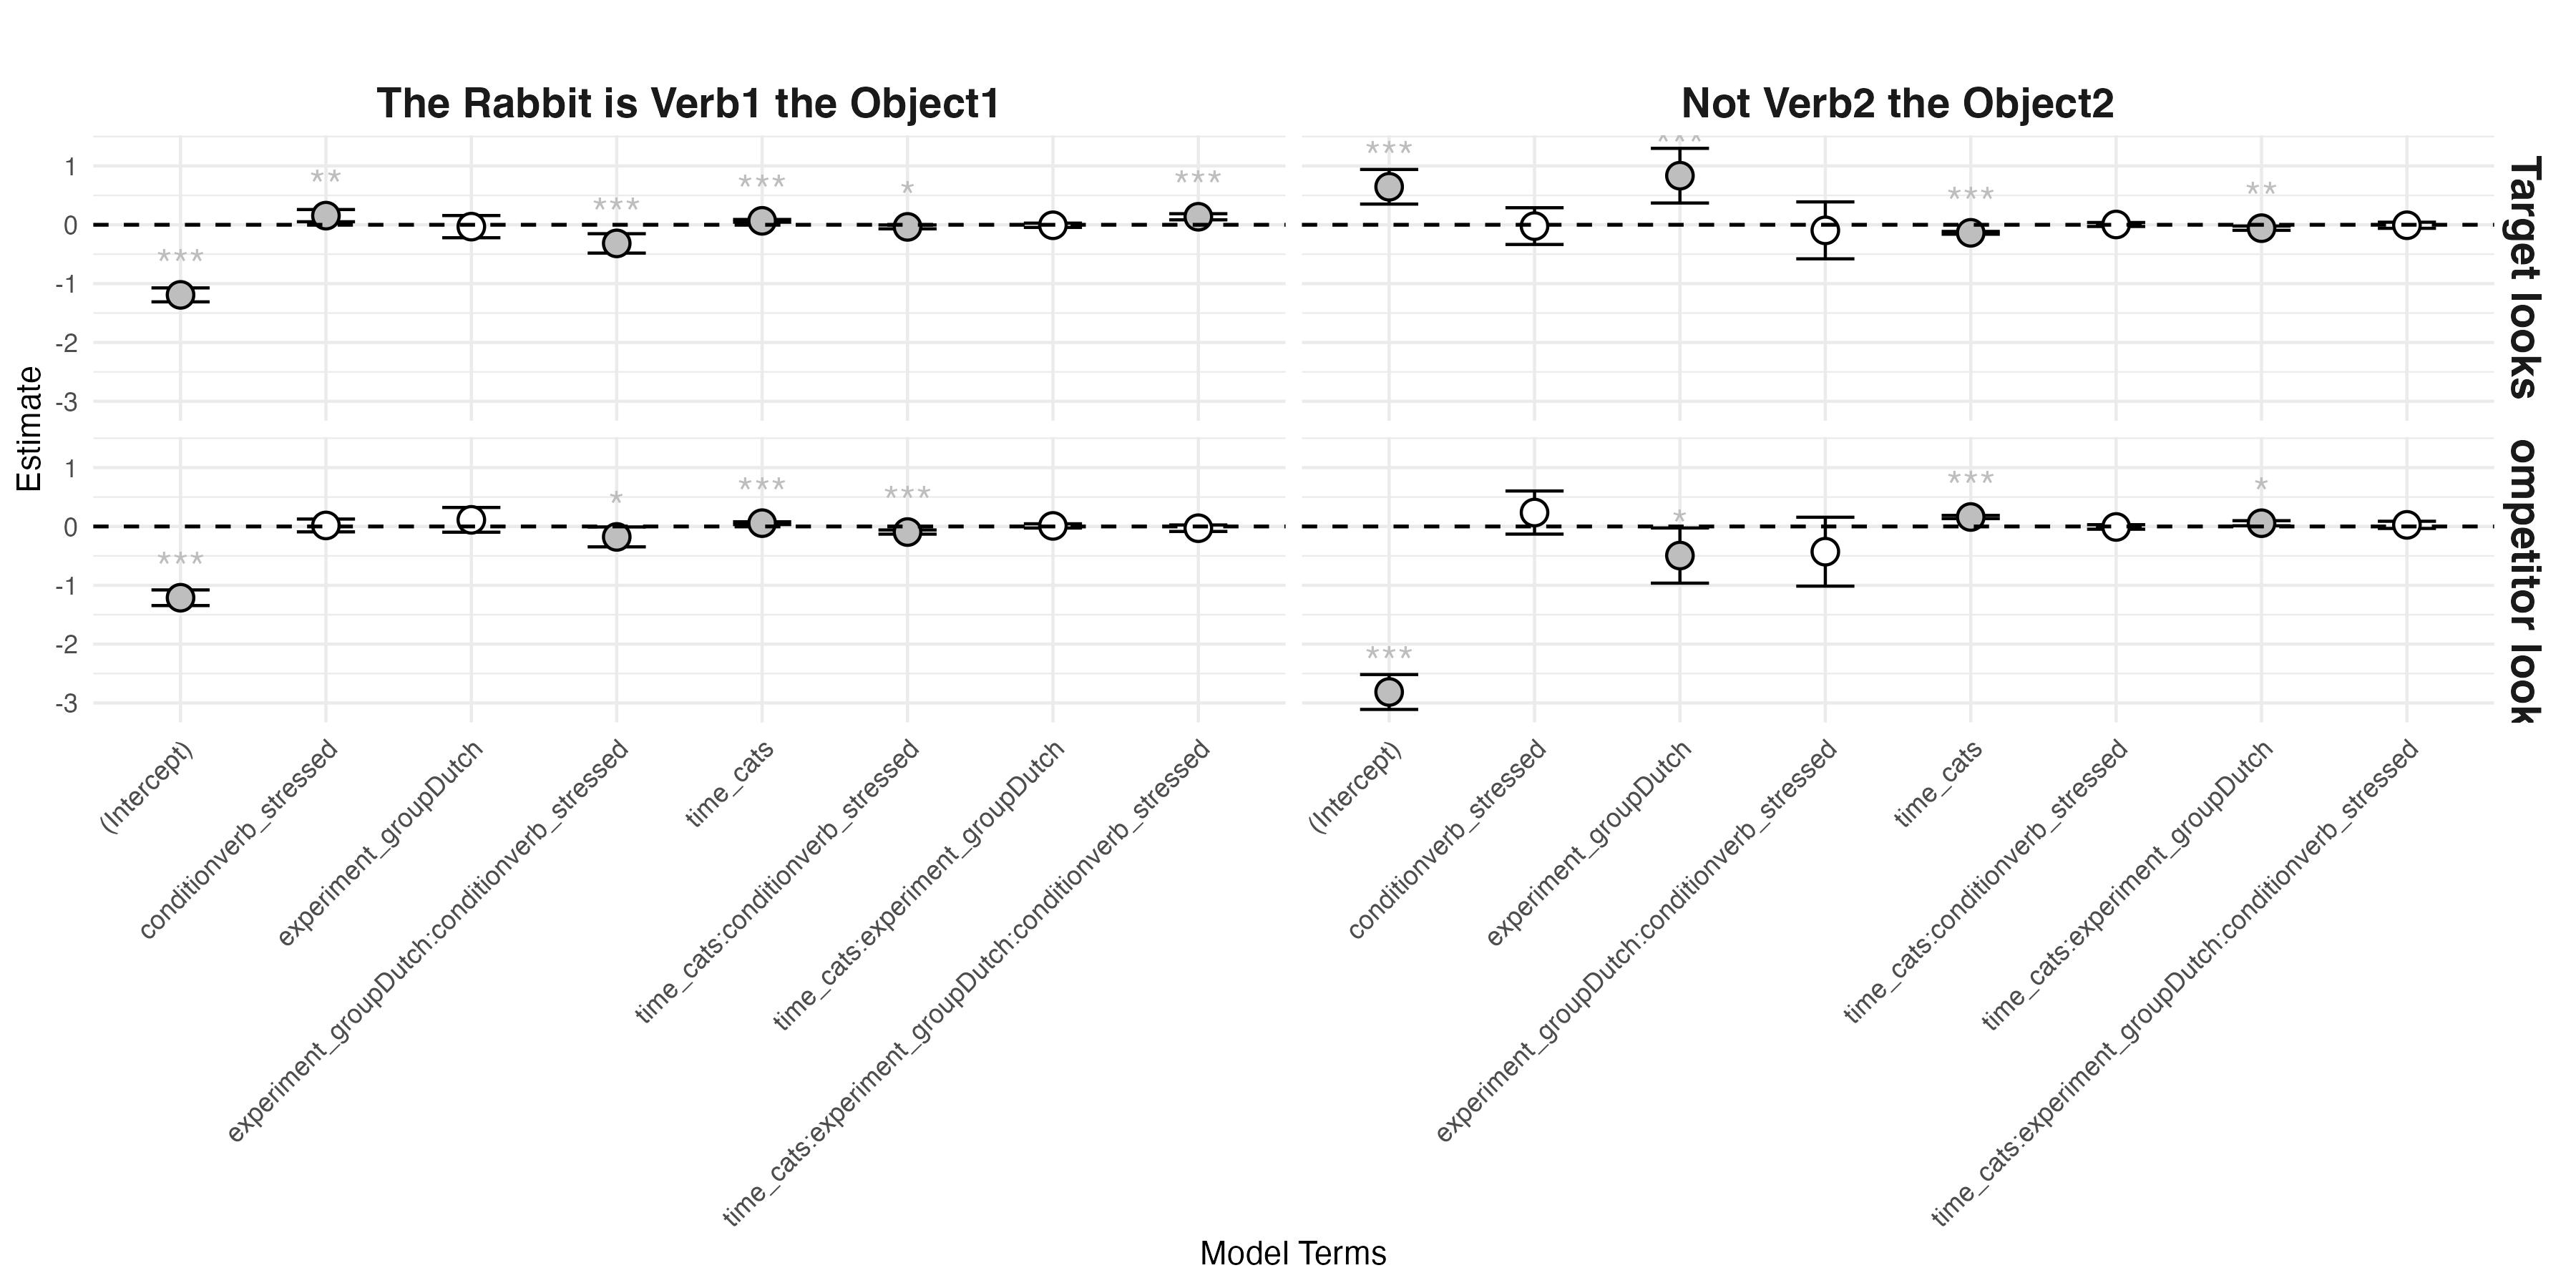
\includegraphics[width=\textwidth,height=\textheight,keepaspectratio]{viz/id_gam_mod_out.png}
    \caption{describe what is going on here- colorized by individual difference measure. Only significant variables are colored (white indicates non-significance). Grey indicates significant but not and individual difference measure}
    \label{fig:id_gam_mod_out}
\end{figure}

L1 

L2


